\documentclass[a4paper]{report}
\usepackage[utf8]{inputenc}
\usepackage[english,turkish]{babel}
\selectlanguage{turkish}
\usepackage{amsmath}
\usepackage{float}
\usepackage{commath}
\usepackage{pst-all}
\usepackage{tikz}
\usepackage{placeins}
\usepackage{flafter}
% Title Page
\title{MAK 524 \emph{Modal Analiz}\\~\\ I. Ödev Çözümleri}
\author{Burak ER}


\begin{document}
\maketitle

%\begin{abstract}
%\end{abstract}

\section*{Hareket Denklemlerinin Çıkarılması}

\subsection*{Taşıt gövdesi kinematik analizi}

Hareket denklemlerinin çıkarılması için taşıtın iki eksende de yaptığı dönmenin tarif edilmesi gerekir. Küçük açılar için dönmenin sırasının değişebileceği bilindiğinden; dönme hareketi ard arda dönme matrisleri ile ifade edilirse bu matrislerin çarpım sırası değiştirilebilir. Bu nedenle:

\begin{eqnarray*}
\left[ \mathbf{A}\right] &=&\left[ \mathbf{A}\right]_x \left[ \mathbf{A}\right]_y \\
\left[ \mathbf{A}\right] &=&\left[ \mathbf{A}\right]_y \left[ \mathbf{A}\right]_x
\end{eqnarray*}
yazılabilir. Burada
\begin{eqnarray*}
\left[ \mathbf{A}\right]_x &=&\left[\begin{array}{ccc} 1 & 0 & 0\\ 0 & \cos\!\left(\mathrm{\phi}\right) & - \sin\!\left(\mathrm{\phi}\right)\\ 0 & \sin\!\left(\mathrm{\phi}\right) & \cos\!\left(\mathrm{\phi}\right) \end{array}\right]\\
\\
\left[ \mathbf{A}\right]_x &=&\left[\begin{array}{ccc} \cos\!\left(\mathrm{\theta}\right) & 0 & \sin\!\left(\mathrm{\theta}\right)\\ 0 & 1 & 0\\ - \sin\!\left(\mathrm{\theta}\right) & 0 & \cos\!\left(\mathrm{\theta}\right) \end{array}\right]
\end{eqnarray*}
küçük açılar için transformasyon matrisleri
\begin{eqnarray*}
\left[ \mathbf{A}\right]_x &=&\left[\begin{array}{ccc} 1 & 0 & 0\\ 0 & 1 & - \phi\\ 0 & \phi & \phi \end{array}\right]\\
\\
\left[ \mathbf{A}\right]_x &=&\left[\begin{array}{ccc} 1 & 0 & \theta\\ 0 & 1 & 0\\ - \theta & 0 & 1 \end{array}\right]
\end{eqnarray*}
olur. Küçük açılar için $\phi \, \theta \approx 0$ alınırsa taşıt gövdesindeki noktaların sabit takıma transformasyonlarının matrisi
\begin{eqnarray*}
\left[ \mathbf{A}\right] &=&\left[\begin{array}{ccc} 1 & 0 & \theta\\ 0 & 1 & - \phi\\ -\theta & \phi & 1 \end{array}\right]
\end{eqnarray*}
taşıt üzerindeki herhangi bir noktanın konumu sabit takımda
\begin{eqnarray*}
\mathbf{r}&=&\mathbf{R}+\left[ \mathbf{A}\right] \mathbf{\bar{u}}
\end{eqnarray*}

\begin{eqnarray*}
\mathbf{r}&=&z\left[\begin{array}{c} 0\\ 0\\ 1\end{array} \right]+\left[\begin{array}{ccc} 1 & 0 & \theta\\ 0 & 1 & - \phi\\ -\theta & \phi & 1 \end{array}\right] \left[\begin{array}{c} \bar{u}_x\\ \bar{u}_y\\ 0\end{array} \right]
\end{eqnarray*}
yazılabilir.Burada sabit takım ile araca gömülü takım başlangıçta çakışık alınmıştır. \\
~\\
Araç üzerindeki süspansiyon bağlantı noktalarının yer değiştirmeleri bulunmak istenirse:\\
~\\
\underline{1 numaralı bağlantı noktasının son konumu:}
\begin{eqnarray*}
\mathbf{r}_1&=&z\left[\begin{array}{c} 0\\ 0\\ 1\end{array} \right]+\left[\begin{array}{ccc} 1 & 0 & \theta\\ 0 & 1 & - \phi\\ -\theta & \phi & 1 \end{array}\right] \left[\begin{array}{c} \bar{u}_x\\ \bar{u}_y\\ 0\end{array} \right]
\\
\\
&=& \left[\begin{array}{c} \bar{u}_{x}\\ \bar{u}_{y}\\ z +\phi \bar{u}_{y} - \theta \bar{u}_{x} \end{array} \right]
\end{eqnarray*}\\
\underline{aynı şekilde diğer yaylar için:}\\
\begin{eqnarray*}
\mathbf{r}_2&=&z\left[\begin{array}{c} 0\\ 0\\ 1\end{array} \right]+\left[\begin{array}{ccc} 1 & 0 & \theta\\ 0 & 1 & - \phi\\ -\theta & \phi & 1 \end{array}\right] \left[\begin{array}{c} -\bar{u}_x\\ \bar{u}_y\\ 0\end{array} \right]
\\
\\
&=& \left[\begin{array}{c} -\bar{u}_{x}\\ \bar{u}_{y}\\ z +\phi \bar{u}_{y} + \theta \bar{u}_{x} \end{array} \right]
\end{eqnarray*}

\begin{eqnarray*}
\mathbf{r}_3&=&z\left[\begin{array}{c} 0\\ 0\\ 1\end{array} \right]+\left[\begin{array}{ccc} 1 & 0 & \theta\\ 0 & 1 & - \phi\\ -\theta & \phi & 1 \end{array}\right] \left[\begin{array}{c} -\bar{u}_x\\ -\bar{u}_y\\ 0\end{array} \right]
\\
\\
&=& \left[\begin{array}{c} -\bar{u}_{x}\\-\bar{u}_{y}\\ z -\phi \bar{u}_{y} + \theta \bar{u}_{x} \end{array} \right]
\end{eqnarray*}
\begin{eqnarray*}
\mathbf{r}_4&=&z\left[\begin{array}{c} 0\\ 0\\ 1\end{array} \right]+\left[\begin{array}{ccc} 1 & 0 & \theta\\ 0 & 1 & - \phi\\ -\theta & \phi & 1 \end{array}\right] \left[\begin{array}{c} \bar{u}_x\\ -\bar{u}_y\\ 0\end{array} \right]
\\
\\
&=& \left[\begin{array}{c} \bar{u}_{x}\\ -\bar{u}_{y}\\ z -\phi \bar{u}_{y} - \theta \bar{u}_{x} \end{array} \right]
\end{eqnarray*}\\
Dolayısıyla her bir noktanın deplasmanları\\
\begin{eqnarray*}
\begin{array}{cc}
\mathbf{u}_1=\left[\begin{array}{c} 0\\ 0\\ z +\phi \bar{u}_{y} - \theta \bar{u}_{x} \end{array} \right]& \mathbf{u}_2=\left[\begin{array}{c} 0\\ 0\\ z +\phi \bar{u}_{y} + \theta \bar{u}_{x} \end{array} \right]
\end{array}
\end{eqnarray*}
\begin{eqnarray*}
\begin{array}{cc}
\mathbf{u}_3=\left[\begin{array}{c} 0\\0\\ z -\phi \bar{u}_{y} + \theta \bar{u}_{x} \end{array} \right]& \mathbf{u}_4=\left[\begin{array}{c} 0\\ 0\\ z -\phi \bar{u}_{y} - \theta \bar{u}_{x} \end{array} \right]
\end{array}
\end{eqnarray*}
bulunur. Yalnızca z bileşenleri alınırsa deplasmanlar
\begin{eqnarray}
\begin{array}{cc}
u_1= z +\phi \bar{u}_{y} - \theta \bar{u}_{x} \\ 
u_2= z +\phi \bar{u}_{y} + \theta \bar{u}_{x} \\
u_3= z -\phi \bar{u}_{y} + \theta \bar{u}_{x} \\
u_4= z -\phi \bar{u}_{y} - \theta \bar{u}_{x} \\
\end{array}
\label{suspensiyon_tasit_uzerindeki_deplasmanlar}
\end{eqnarray}
bulunur. Her iki tarafı zamana göre türeterek bu deplasmanların hızları da aşağıdaki gibi elde edilir.
\begin{eqnarray}
\begin{array}{cc}
\dot{u}_1= \dot{z} +\dot{\phi} \bar{u}_{y} - \dot{\theta} \bar{u}_{x} \\ 
\dot{u}_2= \dot{z} +\dot{\phi} \bar{u}_{y} + \dot{\theta} \bar{u}_{x} \\
\dot{u}_3= \dot{z} -\dot{\phi} \bar{u}_{y} + \dot{\theta} \bar{u}_{x} \\
\dot{u}_4= \dot{z} -\dot{\phi} \bar{u}_{y} - \dot{\theta} \bar{u}_{x} \\
\end{array}
\label{suspensiyon_tasit_uzerindeki_hizlar}
\end{eqnarray}\\
Hareket denklemleri için gerekli lokal takımda taşıt açısal hızının skew-symmetric ifadesi:
\begin{eqnarray*}
\mathbf{\tilde{\bar{{\omega}}}}=\mathbf{A}^T \dot{\mathbf{A}}
\end{eqnarray*}
buradan, küçük açıların çarpımların sıfır kabul edilmesiyle lokal takımda açısal hız
\begin{eqnarray*}
\mathbf{{\bar{{\omega}}}}=\left[ \begin{array}{c}\dot{\phi} \\ \dot{\theta} \\0\end{array}\right]
\end{eqnarray*}
bulunur. Aynı şekilde açısal hız 
\begin{eqnarray*}
\mathbf{{\bar{{\alpha}}}}=\left[ \begin{array}{c}\ddot{\phi} \\ \ddot{\theta} \\0\end{array}\right]
\end{eqnarray*}
olarak elde edilir.
\subsubsection*{Taşıt kinetik analizi}
Taşıt hareketi 7 adet bağımsız hareket denklemleri ile incelenebilir. Bunlar taşıt gövdesinin 2 adet dönme, 1 adet ötelenme, 4 adet lastiğin ötelenme hareket denklemleridir. Bunlar;\\ \\
\underline{Taşıt dönme ve ötelenme hareket denklemi:}
\begin{eqnarray*}
\sum_{i=0}^{n} \mathbf{ \bar{M}} &=& \mathbf{\bar{I}} \dot{\mathbf{\bar{ \omega}}} - {\mathbf{\bar {\omega}}} \times \mathbf{\bar{I}} \mathbf{\bar{ \omega}}
\end{eqnarray*}
\begin{eqnarray*}
\sum_{i=0}^{n} F_z = m \ddot{z}
\end{eqnarray*}\\
\underline{Tekerlek ötelenme hareket denklemleri:}
\begin{eqnarray*}
\sum_{i=0}^{n} F_{t1} = m \ddot{u}_{t1}\\
\sum_{i=0}^{n} F_{t2} = m \ddot{u}_{t2}\\
\sum_{i=0}^{n} F_{t3} = m \ddot{u}_{t3}\\
\sum_{i=0}^{n} F_{t4} = m \ddot{u}_{t4}
\end{eqnarray*}\\
Sistemdeki tüm kuvvetler
\begin{eqnarray*}
F_1 &=& -k\left(z +\phi \bar{u}_{y} - \theta \bar{u}_{x} - u_{t1}\right)-b \left(\dot{z} +\dot{\phi} \bar{u}_{y} - \dot{\theta} \bar{u}_{x} -\dot{u}_{t1}\right)\\
F_2 &=& -k\left(z +\phi \bar{u}_{y} + \theta \bar{u}_{x} - u_{t2}\right)-b \left(\dot{z} +\dot{\phi} \bar{u}_{y} + \dot{\theta} \bar{u}_{x}-\dot{u}_{t2}\right)\\
F_3 &=& -k\left(z -\phi \bar{u}_{y} + \theta \bar{u}_{x} - u_{t3}\right)-b \left(\dot{z} -\dot{\phi} \bar{u}_{y} + \dot{\theta} \bar{u}_{x}-\dot{u}_{t3}\right)\\
F_4 &=& -k\left(z -\phi \bar{u}_{y} - \theta \bar{u}_{x} - u_{t3}\right)-b \left(\dot{z} -\dot{\phi} \bar{u}_{y} - \dot{\theta} \bar{u}_{x}-\dot{u}_{t4}\right)\\
F_{t1} &=& k\left(z +\phi \bar{u}_{y} - \theta \bar{u}_{x} - u_{t1}\right)+b \left(\dot{z} +\dot{\phi} \bar{u}_{y} - \dot{\theta} \bar{u}_{x}-\dot{u}_{t1}\right) - k_t \left(u_{t1}-z_{r1}\right)\\
F_{t2} &=& k\left(z +\phi \bar{u}_{y} + \theta \bar{u}_{x} - u_{t2}\right)+b \left(\dot{z} +\dot{\phi} \bar{u}_{y} + \dot{\theta} \bar{u}_{x}-\dot{u}_{t2}\right) - k_t \left(u_{t2}-z_{r2}\right)\\
F_{t3} &=& k\left(z -\phi \bar{u}_{y} + \theta \bar{u}_{x} - u_{t3}\right)+b \left(\dot{z} -\dot{\phi} \bar{u}_{y} + \dot{\theta} \bar{u}_{x}-\dot{u}_{t3}\right) - k_t \left(u_{t3}-z_{r3}\right)\\
F_{t4} &=& k\left(z -\phi \bar{u}_{y} - \theta \bar{u}_{x} - u_{t4}\right)+b \left(\dot{z} -\dot{\phi} \bar{u}_{y} - \dot{\theta} \bar{u}_{x}-\dot{u}_{t4}\right) - k_t \left(u_{t4}-z_{r4}\right)\\
\end{eqnarray*}
$F_1$ , $F_2$ , $F_3$ , $F_4$ kuvvetlerinin momentleri ve onların araç koordinat takımındaki ifadeleri, moment alırken aracın dönmesi ihmal edilirse(küçük açılar için):
\begin{eqnarray*}
\mathbf{M}_1&=&\left[\begin{array}{c}
 \bar{u}_{y}\, \left(k\, \left(u_{t1} - z - \phi\, \bar{u}_{y} + \theta\, \bar{u}_{x}\right) + b \, \left(\mathrm{\dot{u}}_{t1} - \dot{z} - \dot{\phi}\, \bar{u}_{y} + \mathrm{\dot{\theta}}\, \bar{u}_{x}\right)\right)
\\ 
-\bar{u}_{x}\, \left(k\, \left(u_{t1} - z - \phi\, \bar{u}_{y} + \theta\, \bar{u}_{x}\right) + b \, \left(\mathrm{\dot{u}}_{t1} - \dot{z} - \dot{\phi}\, \bar{u}_{y} + \mathrm{\dot{\theta}}\, \bar{u}_{x}\right)\right)
\\
 0 \end{array} \right]
\end{eqnarray*}

\begin{eqnarray*}
\mathbf{M}_2&=&\left[\begin{array}{c}
 -\bar{u}_{y}\, \left(k\, \left(z - u_{t2} + \phi\, \bar{u}_{y} + \theta\, \bar{u}_{x}\right) + b \, \left(\mathrm{\dot{z}-\dot{u}}_{t2} + \dot{\phi}\, \bar{u}_{y} + \mathrm{\dot{\theta}}\, \bar{u}_{x}\right)\right)
\\ 
-\bar{u}_{x}\, \left(k\, \left( z-u_{t2} + \phi\, \bar{u}_{y} + \theta\, \bar{u}_{x}\right) + b\, \left( \dot{z}-\mathrm{\dot{u}}_{t2} + \dot{\phi}\, \bar{u}_{y} + \mathrm{\dot{\theta}}\, \bar{u}_{x}\right)\right)
\\
 0 \end{array} \right]
\end{eqnarray*}

\begin{eqnarray*}
\mathbf{M}_3&=&\left[\begin{array}{c}
 -\bar{u}_{y}\, \left(k\, \left(u_{t3} - z + \phi\, \bar{u}_{y} - \theta\, \bar{u}_{x}\right) + b \, \left(\mathrm{\dot{u}}_{t3} - \dot{z} + \dot{\phi}\, \bar{u}_{y} - \mathrm{\dot{\theta}}\, \bar{u}_{x}\right)\right)
\\ 
\bar{u}_{x}\, \left(k\, \left(u_{t3} - z + \phi\, \bar{u}_{y} - \theta\, \bar{u}_{x}\right) + b \, \left(\mathrm{\dot{u}}_{t3} - \dot{z} + \dot{\phi}\, \bar{u}_{y} - \mathrm{\dot{\theta}}\, \bar{u}_{x}\right)\right)
\\
 0 \end{array} \right]
\end{eqnarray*}

\begin{eqnarray*}
\mathbf{M}_4&=&\left[\begin{array}{c}
- \bar{u}_{y}\, \left(k\, \left(u_{t4} - z + \phi\, \bar{u}_{y} + \theta\, \bar{u}_{x}\right) + b\, \left(\mathrm{\dot{u}}_{t4} - \dot{z} + \dot{\phi}\, \bar{u}_{y}+ \mathrm{\dot{\theta}}\, \bar{u}_{x}\right)\right)
\\ 
-\bar{u}_{x}\, \left(k\, \left(u_{t4} - z + \phi\, \bar{u}_{y} + \theta\, \bar{u}_{x}\right) + b\, \left(\mathrm{\dot{u}}_{t4} - \dot{z} + \dot{\phi}\, \bar{u}_{y}+ \mathrm{\dot{\theta}}\, \bar{u}_{x}\right)\right)
\\
 0 \end{array} \right]
\end{eqnarray*}\\
Tüm kuvvetler hareket denklemlerine konur ve denklemler $\mathbf{M}\ddot{\mathbf{x}} + \mathbf{B} \dot{\mathbf{x}}+\mathbf{K}\mathbf{x}=\mathbf{F}$ formunda yazılırsa,
\begin{eqnarray*}
\mathbf{M}&=&\left[ 
\begin{array}{ccccccc}
m&0&\cdots&&&&0\\
&I_{xx}&0&\cdots&&&\vdots\\
&&I_{yy}&0&\cdots&&0\\
&&&m_{t1}&0&&\vdots\\
&symmetric&&&m_{t2}&0&\vdots\\
&&&&&m_{t3}&0\\
&&&&&&m_{t4}\\
\end{array} \right]
\end{eqnarray*}

\begin{eqnarray*}
\mathbf{B}&=&\left[ 
\begin{array}{ccccccc}
4b&0&0&-b&-b&-b&-b\\
0&4b\bar{u}_y^2&0&-b\bar{u}_y&-b\bar{u}_y&b\bar{u}_y&b\bar{u}_y\\
0&0&4b\bar{u}_x^2&b\bar{u}_x&-b\bar{u}_x&-b\bar{u}_x&b\bar{u}_x\\
-b&-b\bar{u}_y&b\bar{u}_x&b&0&0&0\\
-b&-b\bar{u}_y&-b\bar{u}_x&0&b&0&0\\
-b&b\bar{u}_y&-b\bar{u}_x&0&0&b&0\\
-b&b\bar{u}_y&b\bar{u}_x&0&0&0&b\\
\end{array} \right]
\end{eqnarray*}
\begin{eqnarray*}
\mathbf{K}&=&\left[ 
\begin{array}{ccccccc}
4k&0&0&-k &-k &-k&-k\\
0&4k\bar{u}_y^2&0&k\bar{u}_y&k\bar{u}_y&-k\bar{u}_y&-k\bar{u}_y\\
0&0&4k\bar{u}_x^2&k\bar{u}_x&-k\bar{u}_x&-k\bar{u}_x&k\bar{u}_x\\
-k&-k\bar{u}_y&k\bar{u}_x&k+k_t&0&0&0\\
-k&-k\bar{u}_y&-k\bar{u}_x&0&k+k_t&0&0\\
-k&k\bar{u}_y&-k\bar{u}_x&0&0&k+k_t&0\\
-k&k\bar{u}_y&k\bar{u}_x&0&0&0&k+k_t\\
\end{array} \right]
\end{eqnarray*}
\begin{eqnarray*}
\mathbf{F}&=&
\left[
\begin{array}{c}
0\\
0\\
0\\
k_t z_{r1}\\
k_t z_{r2}\\
k_t z_{r3}\\
k_t z_{r4}
\end{array}
\right]
\end{eqnarray*}
\\
bulunur. Verilen değerler  $m=1000 kg$, $b=16000 \frac{Ns}{m}$, $k=16000 \frac{N}{m}$,   $k_t=160000 \frac{N}{m}$ yerine konursa örnek taşıt için kütle, sönüm ve katılık matrisleri:
\begin{eqnarray*}
\mathbf{M}&=&\left[ 
\begin{array}{ccccccc}
1000&0&\cdots&&&&0\\
&2300&0&\cdots&&&\vdots\\
&&5300&0&\cdots&&0\\
&&&45&0&&\vdots\\
&symmetric&&&45&0&\vdots\\
&&&&&45&0\\
&&&&&&45\\
\end{array} \right]
\end{eqnarray*}

\begin{eqnarray*}
\mathbf{B}&=&\left[\begin{array}{ccccccc} 4000 & 0 & 0 & -1000 & -1000 & -1000 & -1000\\ 0 & 16000 & 0 & -1000 & -1000 & 1000 & 1000\\ 0 & 0 & 4000 & 2000 & -2000 & -2000 & 2000\\ -1000 & -1000 & 2000 & 1000 & 0 & 0 & 0\\ -1000 & -1000 & -2000 & 0 & 1000 & 0 & 0\\ -1000 & 1000 & -2000 & 0 & 0 & 1000 & 0\\ -1000 & 1000 & 2000 & 0 & 0 & 0 & 1000 \end{array}\right]
\end{eqnarray*}
\begin{eqnarray*}
\mathbf{K}&=&
\left[\begin{array}{ccccccc} 64000 & 0 & 0 & -16000 & -16000 & -16000 & -16000\\ 0 & 256000 & 0 & -16000 & -16000 & 16000 & 16000\\ 0 & 0 & 64000 & 32000 & -32000 & -32000 & 32000\\ -16000 & -16000 & 32000 & 176000 & 0 & 0 & 0\\ -16000 & -16000 & -32000 & 0 & 176000 & 0 & 0\\ -16000 & 16000 & -32000 & 0 & 0 & 176000 & 0\\ -16000 & 16000 & 32000 & 0 & 0 & 0 & 176000 \end{array}\right]
\end{eqnarray*}
\begin{eqnarray*}
\mathbf{F}&=&
\left[
\begin{array}{c}
0\\
0\\
0\\
160000 z_{r1}\\
160000 z_{r2}\\
160000 z_{r3}\\
160000 z_{r4}
\end{array}
\right]
\end{eqnarray*}
\\
~\\
\begin{center}
\clearpage
\section*{Çözümler}
\end{center}


\subsection*{1.	Sönümlü ve Sönümsüz hal için doğal frekansları ve titreşim modlarını bulunuz.}
Kolaylaştırma açısından vizkoz sönüm yapısal sönüm olarak alınırsa, hareket denklemleri
\begin{eqnarray*}
\mathbf{M} \ddot{\mathbf{x}}+\left(\mathbf{K}+i \mathbf{B}\right)\mathbf{x}=\mathbf{F}
\end{eqnarray*}
olarak elde edilir.\\
~\\
Çok serbestlik dereceli sistem halinde özdeğer problemi
\begin{eqnarray*}
\left(\mathbf{M}^{-1} {\mathbf{{K}}}_c-\lambda^2 \right)\mathbf{u}=\mathbf{0}
\end{eqnarray*}\\
olarak ifade edilebilir. \\
~\\
\underline{Sönümsüz hal doğal frekansları:}\\
~\\
Sönümsüz halde $\mathbf{B}=0$ alınarak özdeğer problemi çözülürse, taşıt modeli için özdeğerler ve öz vektörler \emph{Matlab} programı yardımıyla
\begin{eqnarray*}
\mathbf{\Omega}=\left[\begin{array}{ccccccc} 7.6219 & 0 & 0 & 0 & 0 & 0 & 0\\ 0 & 62.586 & 0 & 0 & 0 & 0 & 0\\ 0 & 0 & 10.426 & 0 & 0 & 0 & 0\\ 0 & 0 & 0 & 62.56 & 0 & 0 & 0\\ 0 & 0 & 0 & 0 & 2.7705 & 0 & 0\\ 0 & 0 & 0 & 0 & 0 & 62.539 & 0\\ 0 & 0 & 0 & 0 & 0 & 0 & 62.574 \end{array}\right]
\end{eqnarray*}
\begin{eqnarray*}
\mathbf{\Psi}=\left[\begin{array}{ccccccc} -0.98339 & 0.0083049 & 0 &0 & 0 & 0 & 0\\ 0 & 0 & 0.98296 & 0.003659 &0 & 0 & 0\\ 0 &0 & 0 & 0 & 0.93958 & 0 & 0.0030935\\ -0.090747 & -0.49998 & 0.091914 & -0.5 & -0.17117 & -0.5 & 0.5\\ -0.090747 & -0.49998 & 0.091914 & -0.5 & 0.17117 & 0.5 & -0.5\\ -0.090747 & -0.49998 & -0.091914 & 0.5 & 0.17117 & -0.5 & -0.5\\ -0.090747 & -0.49998 & -0.091914 & 0.5 & -0.17117 & 0.5 & 0.5 \end{array}\right]
\end{eqnarray*}
~\\
\underline{Sönümlü hal doğal frekansları:}\\
~\\
Sönüm matrisi $\mathbf{B}$ modelde bulunan matris olarak alınıp $\mathbf{K}_c=\mathbf{K}+i\mathbf{B}$ olmak üzere özdeğer problemi yazılırsa
\begin{eqnarray*}
\mathbf{\Omega}=\left[
\begin{array}{ccccccc} 7.6 + 0.22\, \mathrm{i} & 0 & 0 & 0 & 0 & 0 & 0\\ 0 & 63.0 + 0.18\, \mathrm{i} & 0 & 0 & 0 & 0 & 0\\ 0 & 0 & 10.0 + 0.32\, \mathrm{i} & 0 & 0 & 0 & 0\\ 0 & 0 & 0 & 63.0 + 0.18\, \mathrm{i} & 0 & 0 & 0\\ 0 & 0 & 0 & 0 & 2.8 + 0.041\, \mathrm{i} & 0 & 0\\ 0 & 0 & 0 & 0 & 0 & 63.0 + 0.18\, \mathrm{i} & 0\\ 0 & 0 & 0 & 0 & 0 & 0 & 63.0 + 0.18\, \mathrm{i} \end{array}\right]
\end{eqnarray*}
\begin{eqnarray*}
\begin{array}{cc} \Psi_1=\left[
\begin{array}{c} 0.98\\ 0\\ 0\\ 0.091 + 5.2\cdot 10^{-3}\, \mathrm{i}\\ 0.091 + 5.2\cdot 10^{-3}\, \mathrm{i}\\ 0.091 + 5.2\cdot 10^{-3}\, \mathrm{i}\\ 0.091 + 5.2\cdot 10^{-3}\, \mathrm{i} \end{array}\right]&
\Psi_2=\left[\begin{array}{c} -8.3\cdot 10^{-3} - 4.8\cdot 10^{-4}\, \mathrm{i}\\ 0\\ 0\\ 0.5\\ 0.5\\ 0.5\\ 0.5 \end{array}\right]\\\\
\Psi_3=\left[\begin{array}{c} 0\\ 0.98\\ 0\\ 0.092 + 5.4\cdot 10^{-3}\, \mathrm{i}\\ 0.092 + 5.4\cdot 10^{-3}\, \mathrm{i}\\ -0.092 - 5.4\cdot 10^{-3}\, \mathrm{i}\\ -0.092 - 5.4\cdot 10^{-3}\, \mathrm{i} \end{array}\right]&
\Psi_4=\left[\begin{array}{c} 0\\ 3.7\cdot 10^{-3} + 2.1\cdot 10^{-4}\, \mathrm{i}\\ 0\\ -0.5 - 8.9\cdot 10^{-14}\, \mathrm{i}\\ -0.5 - 5.9\cdot 10^{-14}\, \mathrm{i}\\ 0.5 + 1.4\cdot 10^{-13}\, \mathrm{i}\\ 0.5 \end{array}\right]\\\\
\Psi_5=\left[\begin{array}{c} 0\\ 0\\ 0.94\\ -0.17 - 9.7\cdot 10^{-3}\, \mathrm{i}\\ 0.17 + 9.7\cdot 10^{-3}\, \mathrm{i}\\ 0.17 + 9.7\cdot 10^{-3}\, \mathrm{i}\\ -0.17 - 9.7\cdot 10^{-3}\, \mathrm{i} \end{array}\right]&
\Psi_6=\left[\begin{array}{c} 0\\ 0\\ -3.1\cdot 10^{-3} - 1.8\cdot 10^{-4}\, \mathrm{i}\\ -0.5 - 4.8\cdot 10^{-14}\, \mathrm{i}\\ 0.5 + 8.4\cdot 10^{-14}\, \mathrm{i}\\ 0.5\\ -0.5 - 4.0\cdot 10^{-14}\, \mathrm{i} \end{array}\right]\\\\
\Psi_7=\left[\begin{array}{c} 0\\ 0\\ 0\\ -0.5 - 2.2\cdot 10^{-14}\, \mathrm{i}\\ 0.5\\ -0.5 + 1.3\cdot 10^{-14}\, \mathrm{i}\\ 0.5 + 8.5\cdot 10^{-15}\, \mathrm{i} \end{array}\right]\end{array}
\end{eqnarray*}\\
Görüldüğü üzere doğal frekanslar ve mod şekilleri sanal sayılar olarak bulunmuştur. Özdeğerler için sanal kısımlar sönüm miktarını ifade etmektedir.
\subsection*{2.Titreşim modlarının ortogonallik şartlarını sağladığını gösteriniz.}
Titreşim modlarının ortogonallik şartını sağlaması için
\begin{eqnarray*}
\begin{array}{c}
{\Psi}_r^T\mathbf{M}{\Psi}_s=\mathbf{0}\qquad r\neq s\\
{\Psi}_r^T\mathbf{K}{\Psi}_s=\mathbf{0}\qquad r\neq s\\
\end{array}
\end{eqnarray*}\\
eşitliğini sağlaması gerekir. Bu nedenle;
\begin{eqnarray*}
\begin{array}{c}
\mathbf{\Psi}^T\mathbf{M}{\mathbf{\Psi}}=\mathbf{m}\\
\mathbf{\Psi}^T\mathbf{K}{\mathbf{\Psi}}=\mathbf{k}\\
\end{array}
\end{eqnarray*}\\
ifadelerinde $\mathbf{m}$ ve $\mathbf{k}$ matrisleri diagonal olmalıdırlar. Hesaplamalar yapılırsa,\\
~\\
\underline{Sönümsüz hal için}
\begin{eqnarray*}
\bar{ \mathbf{m}}&=&\left[\begin{array}{ccccccc} 988.0 & 0 & 0 & 0 & 0 & 0 & 0\\ 0 & 45.0 & 0 & 0 & 0 & 0 & 0\\ 0 & 0 & 2.2\cdot 10^3 & 0 & 0 & 0 & 0\\ 0 & 0 & 0 & 45.0 & 0 & 0 & 0\\ 0 & 0 & 0 & 0 & 4.7\cdot 10^3 & 0 & 0\\ 0 & 0 & 0 & 0 & 0 & 45.0 & 0\\ 0 & 0 & 0 & 0 & 0 & 0 & 45.0 \end{array}\right]\\
\bar{ \mathbf{k}}&=&\left[\begin{array}{ccccccc} 5.6\cdot 10^4 & 0 & 0 & 0 & 0 & 0 & 0\\ 0 & 1.8\cdot 10^5 & 0 & 0 & 0 & 0 & 0\\ 0 & 0 & 2.4\cdot 10^5 & 0 & 0 & 0 & 0\\ 0 & 0 & 0 & 1.8\cdot 10^5 & 0 & 0 & 0\\ 0 & 0 & 0 & 0 & 3.6\cdot 10^4 & 0 & 0\\ 0 & 0 & 0 & 0 & 0 & 1.8\cdot 10^5 & 0\\ 0 & 0 & 0 & 0 & 0 & 0 & 1.8\cdot 10^5 \end{array}\right]
\end{eqnarray*}
diagonal matrisleri bulunur. Sönümsüz hal için modlar ortogonaldir denir.
\\
~\\
\underline{Sönümlü hal için}\\
\begin{eqnarray*}
\bar{ \mathbf{m}}&=&\left[\begin{array}{ccccccc} 5.6\cdot 10^4 & 0 & 0 & 0 & 0 & 0 & 0\\ 0 & 1.8\cdot 10^5& 0 & 0 & 0 & 0 & 0\\ 0 & 0 & 2.4\cdot 10^5  & 0 & 0 & 0 & 0\\ 0 & 0 & 0 & 1.8\cdot 10^5 & 0 & 0 & 0\\ 0 & 0 & 0 & 0 & 3.6\cdot 10^4 & 0 & 0\\ 0 & 0 & 0 & 0 & 0 & 1.8\cdot 10^5  & 0\\ 0 & 0 & 0 & 0 & 0 & 0 & 1.8\cdot 10^5  \end{array}\right]
\end{eqnarray*}

\begin{eqnarray*}
\bar{ \mathbf{k} }&=&\left[\begin{array}{ccccccc} 5.6\cdot 10^4 & 0 & 0 & 0 & 0 & 0 & 0\\ 0 & 1.8\cdot 10^5  & 0 & 0 & 0 & 0 & 0\\ 0 & 0 & 2.4\cdot 10^5 & 0 & 0 & 0 & 0\\ 0 & 0 & 0 & 1.8\cdot 10^5  & 0 & 0 & 0\\ 0 & 0 & 0 & 0 & 3.6\cdot 10^4  & 0 & 0\\ 0 & 0 & 0 & 0 & 0 & 1.8\cdot 10^5 & 0\\ 0 & 0 & 0 & 0 & 0 & 0 & 1.8\cdot 10^5  \end{array}\right]\\
&&\\
&&+\left[\begin{array}{ccccccc} 0 & 0 & 0 & 0 & 0 & 0 & 0\\ 0 &  8.9\cdot 10^{-16}\, \mathrm{i} & 0 & 0 & 0 & 0 & 0\\ 0 & 0 &  1.4\cdot 10^{-14}\, \mathrm{i} & 0 & 0 & 0 & 0\\ 0 & 0 & 0 & - 2.0\cdot 10^{-15}\, \mathrm{i} & 0 & 0 & 0\\ 0 & 0 & 0 & 0 &  2.8\cdot 10^{-13}\, \mathrm{i} & 0 & 0\\ 0 & 0 & 0 & 0 & 0 & - 1.8\cdot 10^{-15}\, \mathrm{i} & 0\\ 0 & 0 & 0 & 0 & 0 & 0 & - 2.1\cdot 10^{-25}\, \mathrm{i} \end{array}\right]
\end{eqnarray*}
diagonal matrisleri bulunur. Sönümlü hal için de modlar ortogonaldir.

\subsection*{3. Modal kütle ve katılıkları hesaplayınız bunlara bakarak bulduğunuz modların normalize olup olmadığını gösteriniz.}
Modal kütleler ve rijitlikler
\begin{eqnarray*}
\bar{ \mathbf{m}}&=&\mathbf{\Psi}^T\mathbf{M}\mathbf{\Psi}\\
\bar{ \mathbf{k}}&=&\mathbf{\Psi}^T\mathbf{K}\mathbf{\Psi}
\end{eqnarray*}
eşitliklerinden bulunmak istenirse,\\
~\\
\underline{Sönümsüz hal için}\\
\begin{eqnarray*}
\bar{ \mathbf{m}}&=&\left[\begin{array}{ccccccc} 988.0 & 0 & 0 & 0 & 0 & 0 & 0\\ 0 & 45.0 & 0 & 0 & 0 & 0 & 0\\ 0 & 0 & 2.2\cdot 10^3 & 0 & 0 & 0 & 0\\ 0 & 0 & 0 & 45.0 & 0 & 0 & 0\\ 0 & 0 & 0 & 0 & 4.7\cdot 10^3 & 0 & 0\\ 0 & 0 & 0 & 0 & 0 & 45.0 & 0\\ 0 & 0 & 0 & 0 & 0 & 0 & 45.0 \end{array}\right]\\
\bar{ \mathbf{k}}&=&\left[\begin{array}{ccccccc} 5.6\cdot 10^4 & 0 & 0 & 0 & 0 & 0 & 0\\ 0 & 1.8\cdot 10^5 & 0 & 0 & 0 & 0 & 0\\ 0 & 0 & 2.4\cdot 10^5 & 0 & 0 & 0 & 0\\ 0 & 0 & 0 & 1.8\cdot 10^5 & 0 & 0 & 0\\ 0 & 0 & 0 & 0 & 3.6\cdot 10^4 & 0 & 0\\ 0 & 0 & 0 & 0 & 0 & 1.8\cdot 10^5 & 0\\ 0 & 0 & 0 & 0 & 0 & 0 & 1.8\cdot 10^5 \end{array}\right]
\end{eqnarray*}
Her bir mod için doğal frekanslar bulunursa
\begin{eqnarray*}
\omega_i&=&\sqrt{\frac{\bar{k}_i}{\bar{m}_i}}
\end{eqnarray*}
bunların daha önce bulunan doğal frekanslara eşit oldukları görülür.\\
~\\
\underline{Sönümlü hal için}\\
\begin{eqnarray*}
\bar{ \mathbf{m}}&=&\left[\begin{array}{ccccccc} 5.6\cdot 10^4 & 0 & 0 & 0 & 0 & 0 & 0\\ 0 & 1.8\cdot 10^5& 0 & 0 & 0 & 0 & 0\\ 0 & 0 & 2.4\cdot 10^5  & 0 & 0 & 0 & 0\\ 0 & 0 & 0 & 1.8\cdot 10^5 & 0 & 0 & 0\\ 0 & 0 & 0 & 0 & 3.6\cdot 10^4 & 0 & 0\\ 0 & 0 & 0 & 0 & 0 & 1.8\cdot 10^5  & 0\\ 0 & 0 & 0 & 0 & 0 & 0 & 1.8\cdot 10^5  \end{array}\right]
\end{eqnarray*}

\begin{eqnarray*}
\bar{ \mathbf{k} }&=&\left[\begin{array}{ccccccc} 5.6\cdot 10^4 & 0 & 0 & 0 & 0 & 0 & 0\\ 0 & 1.8\cdot 10^5  & 0 & 0 & 0 & 0 & 0\\ 0 & 0 & 2.4\cdot 10^5 & 0 & 0 & 0 & 0\\ 0 & 0 & 0 & 1.8\cdot 10^5  & 0 & 0 & 0\\ 0 & 0 & 0 & 0 & 3.6\cdot 10^4  & 0 & 0\\ 0 & 0 & 0 & 0 & 0 & 1.8\cdot 10^5 & 0\\ 0 & 0 & 0 & 0 & 0 & 0 & 1.8\cdot 10^5  \end{array}\right]\\
&&\\
&&+\left[\begin{array}{ccccccc} 0 & 0 & 0 & 0 & 0 & 0 & 0\\ 0 &  8.9\cdot 10^{-16}\, \mathrm{i} & 0 & 0 & 0 & 0 & 0\\ 0 & 0 &  1.4\cdot 10^{-14}\, \mathrm{i} & 0 & 0 & 0 & 0\\ 0 & 0 & 0 & - 2.0\cdot 10^{-15}\, \mathrm{i} & 0 & 0 & 0\\ 0 & 0 & 0 & 0 &  2.8\cdot 10^{-13}\, \mathrm{i} & 0 & 0\\ 0 & 0 & 0 & 0 & 0 & - 1.8\cdot 10^{-15}\, \mathrm{i} & 0\\ 0 & 0 & 0 & 0 & 0 & 0 & - 2.1\cdot 10^{-25}\, \mathrm{i} \end{array}\right]
\end{eqnarray*}
bulunur. 
\subsection*{4. Sönümsüz hal için serbest titreşim hareket denklemlerini $\mathbf{x}=\mathbf{\Psi}\mathbf{q}$ şeklinde bir dönüşümle ayrıklaştırınız. Yeni oluşacak denklemlerini birbirinden bağımsız olduğunu gösteriniz.}~\\
Dönüşüm
\begin{eqnarray*}
\mathbf{x}=\mathbf{\Psi}\mathbf{q}
\end{eqnarray*}
kullanılırsa, hareket denklemleri
\begin{eqnarray*}
\mathbf{M}\mathbf{\Psi}\ddot{\mathbf{q}} +\mathbf{K}\mathbf{\Psi}\mathbf{q}=\mathbf{F}
\end{eqnarray*}
olarak elde edilir. Her iki taraf mod şekil matrisi transpozu ile çarpılırsa ve
\begin{eqnarray*}
\begin{array}{c}
\mathbf{\Psi}^T\mathbf{M}{\mathbf{\Psi}}=\bar{ \mathbf{m}}\\
\mathbf{\Psi}^T\mathbf{K}{\mathbf{\Psi}}=\bar{ \mathbf{k}}\\
\end{array}
\end{eqnarray*}
için son halde hareket denklemleri
\begin{eqnarray*}
\bar{ \mathbf{m}}\ddot{\mathbf{q}} +\bar {\mathbf{k}}\mathbf{q}=\mathbf{\Psi}^T\mathbf{F}
\end{eqnarray*}
olarak elde edilir. İşlemler yapılırsa
\begin{eqnarray*}
\bar{ \mathbf{m}}&=&\left[\begin{array}{ccccccc} 988.0 & 0 & 0 & 0 & 0 & 0 & 0\\ 0 & 45.0 & 0 & 0 & 0 & 0 & 0\\ 0 & 0 & 2.2\cdot 10^3 & 0 & 0 & 0 & 0\\ 0 & 0 & 0 & 45.0 & 0 & 0 & 0\\ 0 & 0 & 0 & 0 & 4.7\cdot 10^3 & 0 & 0\\ 0 & 0 & 0 & 0 & 0 & 45.0 & 0\\ 0 & 0 & 0 & 0 & 0 & 0 & 45.0 \end{array}\right]\\
\bar{ \mathbf{k}}&=&\left[\begin{array}{ccccccc} 5.6\cdot 10^4 & 0 & 0 & 0 & 0 & 0 & 0\\ 0 & 1.8\cdot 10^5 & 0 & 0 & 0 & 0 & 0\\ 0 & 0 & 2.4\cdot 10^5 & 0 & 0 & 0 & 0\\ 0 & 0 & 0 & 1.8\cdot 10^5 & 0 & 0 & 0\\ 0 & 0 & 0 & 0 & 3.6\cdot 10^4 & 0 & 0\\ 0 & 0 & 0 & 0 & 0 & 1.8\cdot 10^5 & 0\\ 0 & 0 & 0 & 0 & 0 & 0 & 1.8\cdot 10^5 \end{array}\right]
\end{eqnarray*}
\begin{eqnarray*}
\mathbf{\Psi}^T\mathbf{F}&=&\left[\begin{array}{c}  - \left(1.5\cdot 10^3\right)\, \mathrm{zr}_{1} - \left(1.5\cdot 10^3\right)\, \mathrm{zr}_{2} - \left(1.5\cdot 10^3\right)\, \mathrm{zr}_{3} - \left(1.5\cdot 10^3\right)\, \mathrm{zr}_{4}\\  - \left(8.0\cdot 10^3\right)\, \mathrm{zr}_{1} - \left(8.0\cdot 10^3\right)\, \mathrm{zr}_{2} - \left(8.0\cdot 10^3\right)\, \mathrm{zr}_{3} - \left(8.0\cdot 10^3\right)\, \mathrm{zr}_{4}\\ \left(1.5\cdot 10^3\right)\, \mathrm{zr}_{1} + \left(1.5\cdot 10^3\right)\, \mathrm{zr}_{2} - \left(1.5\cdot 10^3\right)\, \mathrm{zr}_{3} - \left(1.5\cdot 10^3\right)\, \mathrm{zr}_{4}\\ \left(8.0\cdot 10^3\right)\, \mathrm{zr}_{3} - \left(8.0\cdot 10^3\right)\, \mathrm{zr}_{2} - \left(8.0\cdot 10^3\right)\, \mathrm{zr}_{1} + \left(8.0\cdot 10^3\right)\, \mathrm{zr}_{4}\\ \left(2.7\cdot 10^3\right)\, \mathrm{zr}_{2} - \left(2.7\cdot 10^3\right)\, \mathrm{zr}_{1} + \left(2.7\cdot 10^3\right)\, \mathrm{zr}_{3} - \left(2.7\cdot 10^3\right)\, \mathrm{zr}_{4}\\ \left(8.0\cdot 10^3\right)\, \mathrm{zr}_{2} - \left(8.0\cdot 10^3\right)\, \mathrm{zr}_{1} - \left(8.0\cdot 10^3\right)\, \mathrm{zr}_{3} + \left(8.0\cdot 10^3\right)\, \mathrm{zr}_{4}\\ \left(8.0\cdot 10^3\right)\, \mathrm{zr}_{1} - \left(8.0\cdot 10^3\right)\, \mathrm{zr}_{2} - \left(8.0\cdot 10^3\right)\, \mathrm{zr}_{3} + \left(8.0\cdot 10^3\right)\, \mathrm{zr}_{4} \end{array}
\right]
\end{eqnarray*}
bulunur. Böylelikle denklemler ayrıştırılmış olmaktadır.
\subsection*{5. Dinamik katılık matrisinin elemanlarını aynı grafikte çizdiriniz. (Yatay eksen frekans($\frac{rad}{s}$), düşey eksen dinamik katılık($\frac{N}{m}$) olmalıdır.)}~\\
\underline{Sönümsüz hal}\\~\\
Dinamik katılık matrisinin ifadesi
\begin{eqnarray*}
\mathbf{Z}\left(\omega\right)&=&\frac{\mathbf{F}\left(\omega\right)}{\mathbf{X}\left(\omega\right)}\\
&=&\mathbf{K}-\omega^2\mathbf{M}
\end{eqnarray*}
Sönümsüz halde $\mathbf{Z}$ matrisi elemanları aynı grafikte çizdirilmesiyle Şekil~\ref{fig:dinamikkatilik}'teki grafik elde edilmiştir.
\begin{figure}[th!]
\shorthandoff{=}
\centerline{
{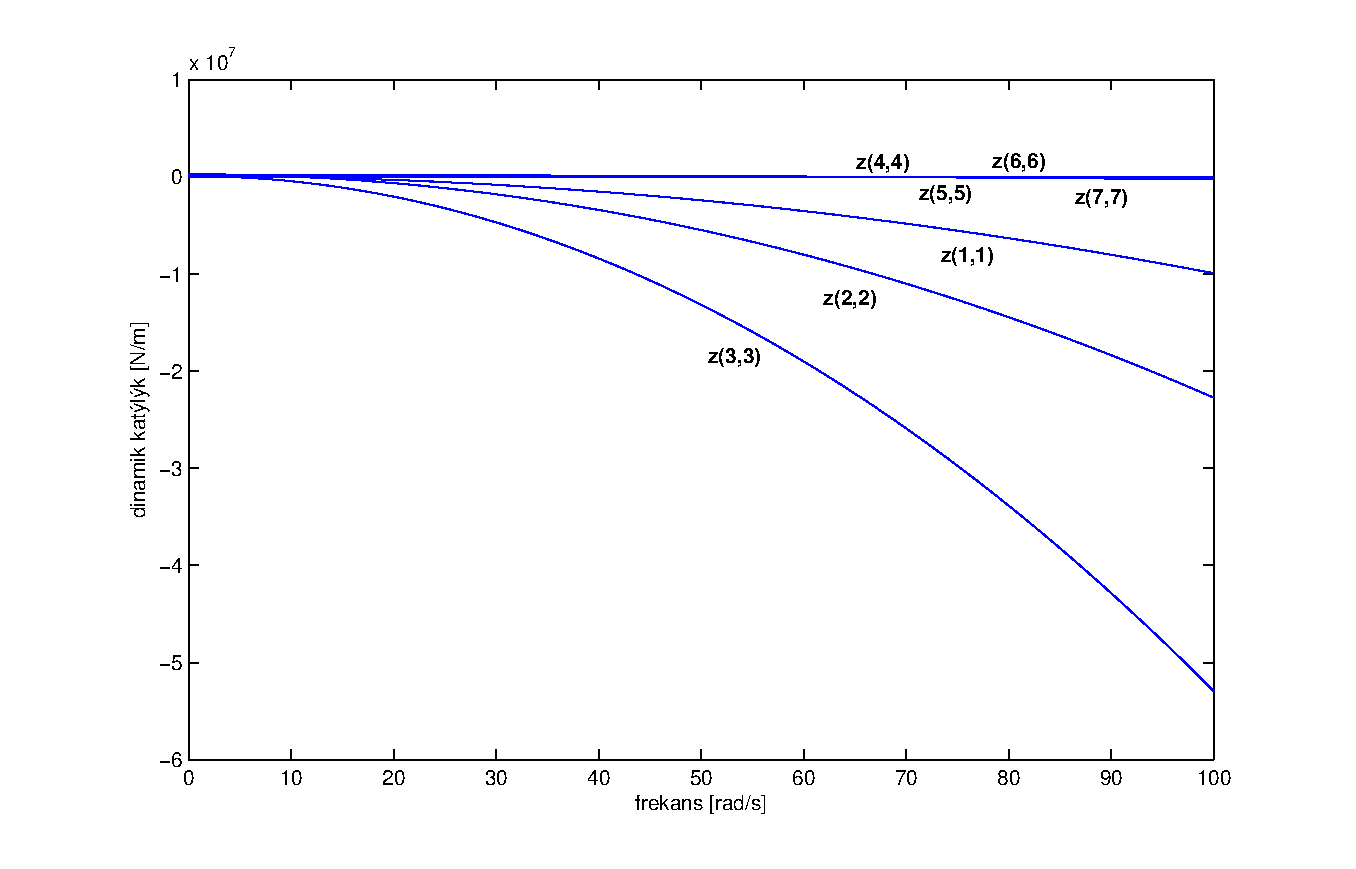
\includegraphics[width=1.3\textwidth]{./dinamikkatilik.eps}}}
\caption[Dinamik katılık]{Sönümsüz hal dinamik katılık elemanlarının çizimi}
\label{fig:dinamikkatilik}
\end{figure}\\
~\\
\underline{Sönümlü hal}\\~\\
Sönümlü halde sistem katılığı $\mathbf{K_c}=\mathbf{K}+i\mathbf{B}$ yazılırsa
\begin{eqnarray*}
\mathbf{Z}\left(\omega\right)&=&\frac{\mathbf{F}\left(\omega\right)}{\mathbf{X}\left(\omega\right)}\\
&=&\mathbf{K}_c-\omega^2\mathbf{M}
\end{eqnarray*}
elde edilir. Grafiği çizildiğinde Şekil~\ref{fig:dinamikkatiliks} elde edilmiştir.
\begin{figure}[H]
\shorthandoff{=}
\centerline{
{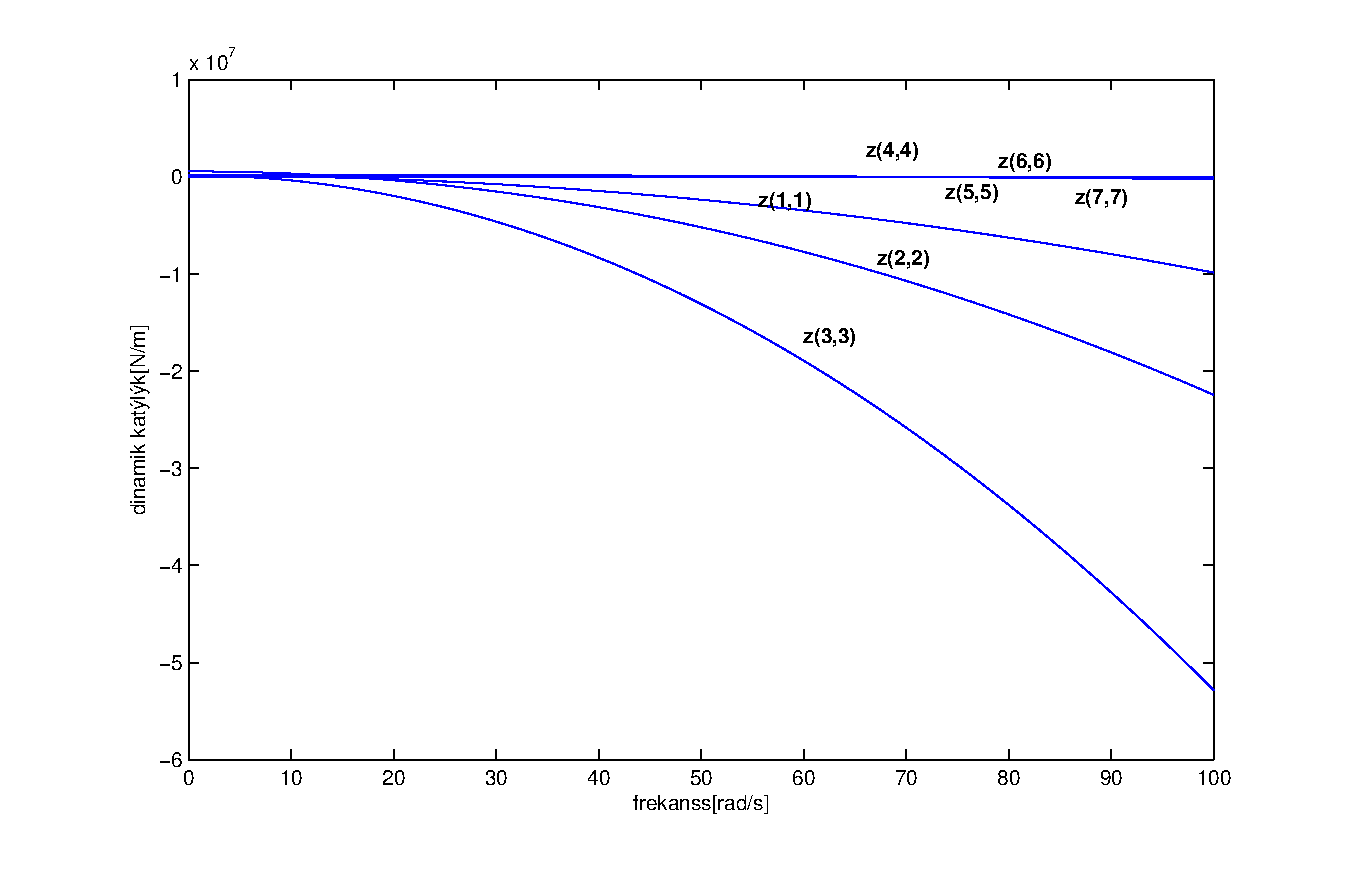
\includegraphics[width=1.3\textwidth]{./dinamikkatiliks.eps}}}
\caption[Dinamik katılık]{Sönümlü hal dinamik katılık elemanlarının çizimi}
\label{fig:dinamikkatiliks}
\end{figure}
\subsection*{6. Reseptans matrisinin tüm elemanlarını aynı grafikte çizdiriniz.a)Tüm reseptansların mutlak değerleri aynı grafikte çizilecek.b)Tüm reseptansların mutlak değerlerinin logaritması aynı grafikte çizdirilecek.}~\\
\underline{Sönümsüz hal için:}\\~\\
Reseptans dinamik katılığın tersi olduğundan 
\begin{eqnarray*}
\mathbf{\alpha}\left(\omega\right)&=&\frac{\mathbf{X}\left(\omega\right)}{\mathbf{F}\left(\omega\right)}\\
&=&\left(\mathbf{K}-\omega^2\mathbf{M}\right)^{-1}
\end{eqnarray*}
yazılabilir.\\~\\
Reseptans matrisinin bileşenlerinin yatay eksen ${rad}/{s}$ ve dikey eksen de ${m}/{N}$ olacak şekilde çizdirdirilmesiyle Şekil~\ref{fig:reseptans} elde edilmiştir.
\begin{figure}[H]
\shorthandoff{=}
\centerline{
{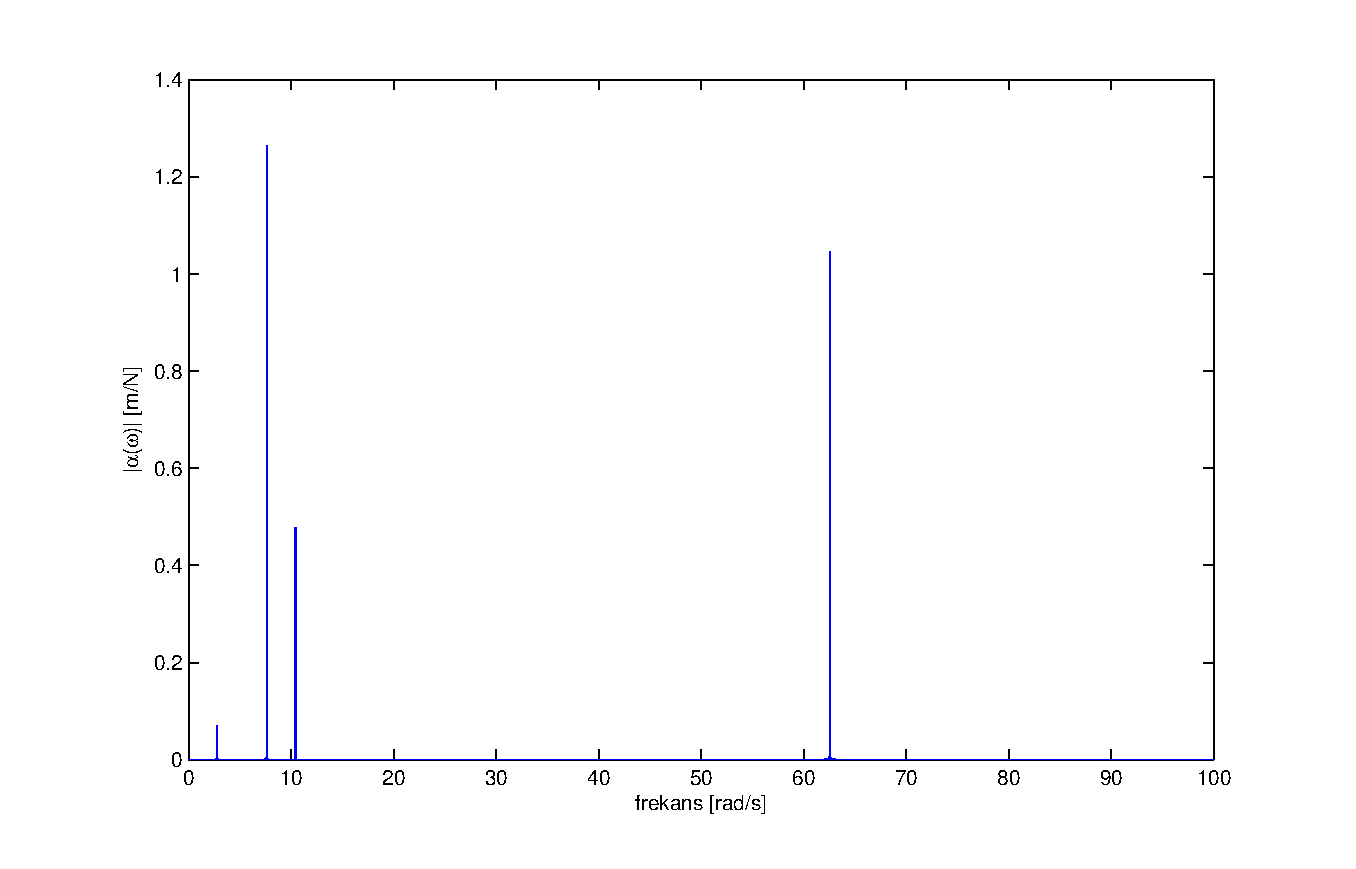
\includegraphics[width=1.3\textwidth]{./reseptans.eps}}}
\caption[Reseptans matrisi elemanları]{Reseptans matrisi elemanları yatay eksen ${rad}/{s}$ ve dikey eksen ${m}/{N}$}
\label{fig:reseptans}
\end{figure}\clearpage~\\
Reseptans matrisinin bileşenlerinin yatay eksen ${rad}/{s}$ ve dikey eksen de $dB$ olacak şekilde çizdirilmesiyle Şekil~\ref{fig:reseptansdb} elde edilmiştir.
\begin{figure}[H]
\shorthandoff{=}
\centerline{
{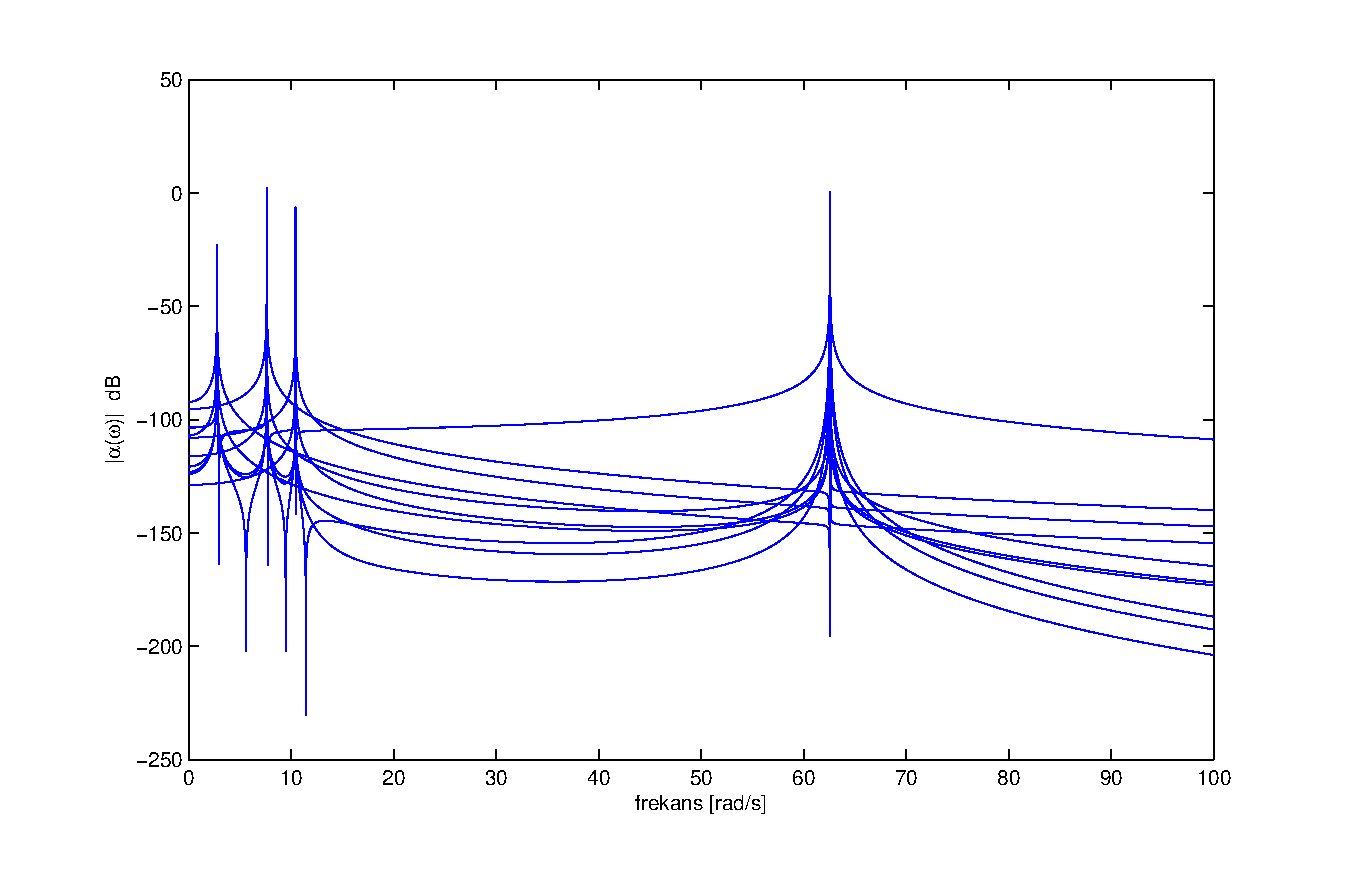
\includegraphics[width=1.3\textwidth]{./reseptansdB.eps}}}
\caption[Reseptans matrisi elemanları]{Reseptans matrisi elemanları yatay eksen ${rad}/{s}$ ve dikey eksen $dB$ }
\label{fig:reseptansdb}
\end{figure}\clearpage~\\
Şekillerden görüldüğü üzere maksimum 4 adet mod belirgindir. Ancak frekansın $\omega\approx62-63 rad/s$ olduğu bölgede birbirine yakın olan modlar bulunmuştur. Bu bölge daha yakından Şekil~\ref{fig:reseptansdbz}' de verilmiştir.
\begin{figure}[H]
\shorthandoff{=}
\centerline{
{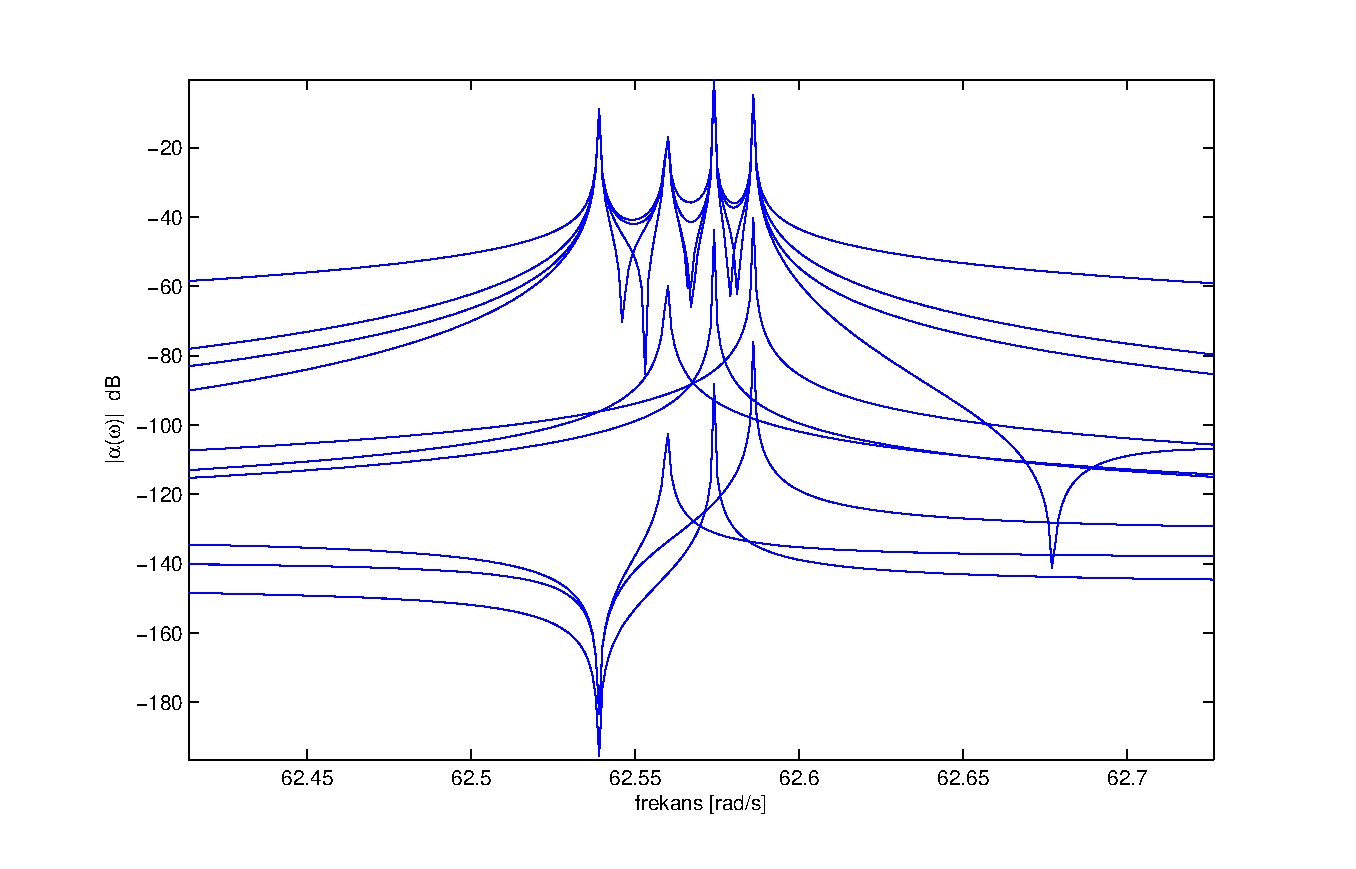
\includegraphics[width=1.3\textwidth]{./reseptansdBz.eps}}}
\caption[Reseptans matrisi elemanları]{Reseptans matrisi elemanlarının $\omega\approx62-63 rad/s$ civarındaki çizgileri. }
\label{fig:reseptansdbz}
\end{figure}
Dolayısıyla beklenildiği üzere 7 serbestlik dereceli sistem için 7 adet rezonans noktası bulunmuştur.\\~\\
\underline{Sönümlü hal için:}
\begin{eqnarray*}
\mathbf{\alpha}\left(\omega\right)&=&\frac{\mathbf{X}\left(\omega\right)}{\mathbf{F}\left(\omega\right)}\\
&=&\left(\mathbf{K}_c-\omega^2\mathbf{M}\right)^{-1}
\end{eqnarray*}
bulunur. Sönümsüz halde çizilen reseptans grafiklerinin sönümlü hal için olanları Şekil~\ref{fig:reseptanss}-\ref{fig:reseptanssdbz}'de verilmiştir.
\clearpage
\begin{figure}[H]
\shorthandoff{=}
\centerline{
{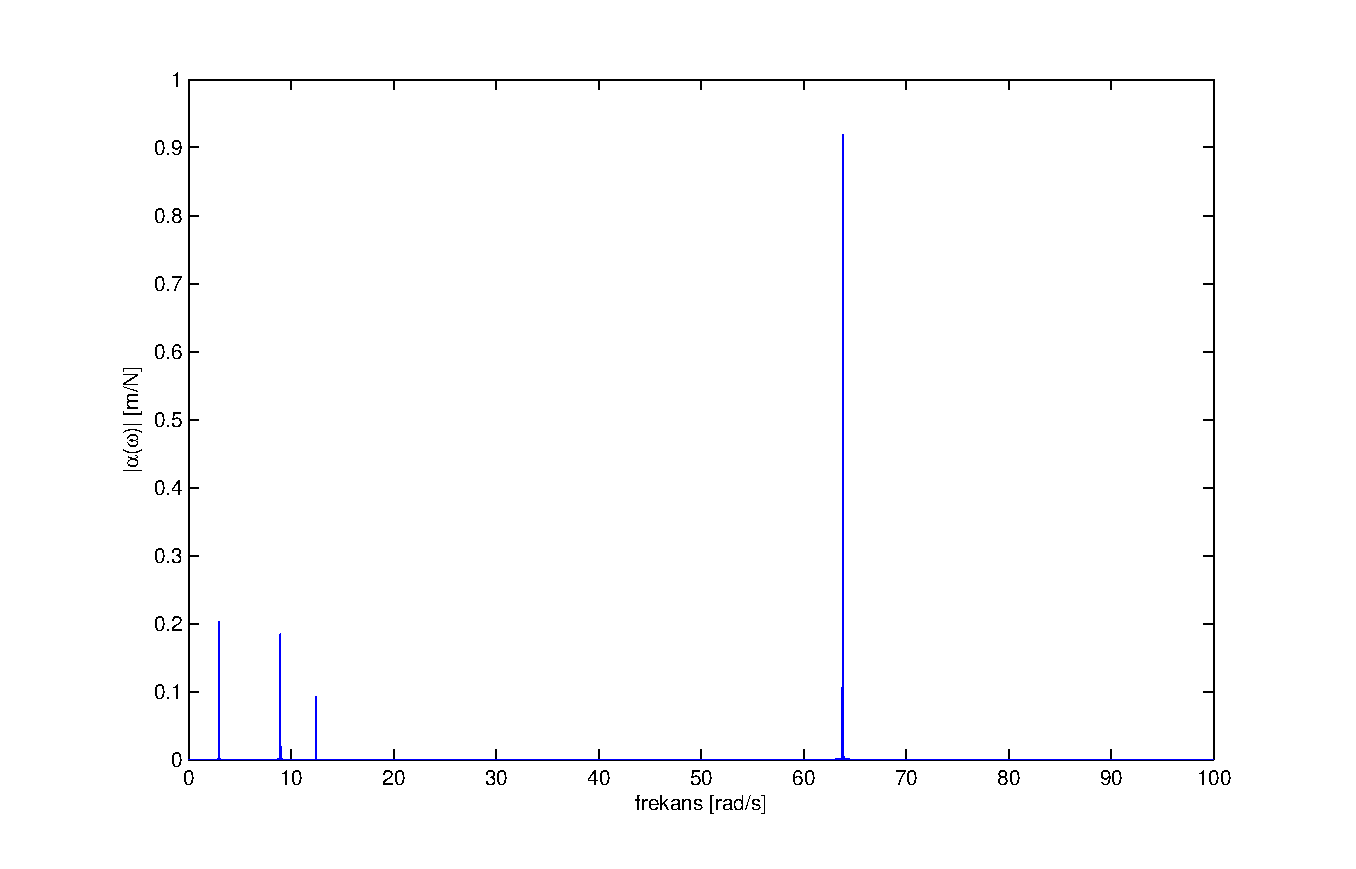
\includegraphics[width=1.3\textwidth]{./reseptanss.eps}}}
\caption[Sönümlü hal reseptans matrisi elemanları]{Sönümlü hal reseptans matrisi elemanları yatay eksen ${rad}/{s}$ ve dikey eksen ${m}/{N}$}
\label{fig:reseptanss}
\end{figure}
~\\
\begin{figure}[H]
\shorthandoff{=}
\centerline{
{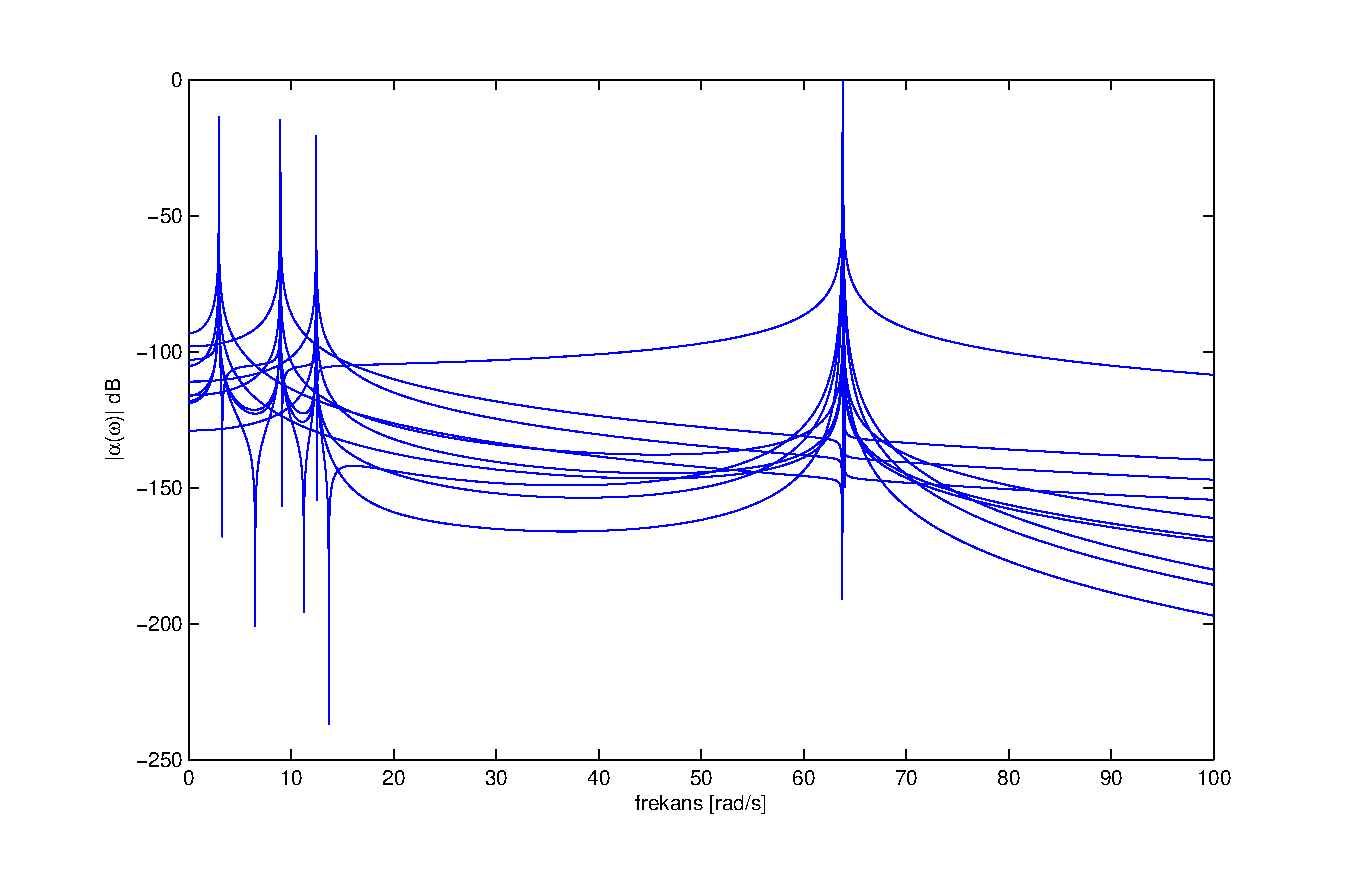
\includegraphics[width=1.3\textwidth]{./reseptanssdB.eps}}}
\caption[Sönümlü hal reseptans matrisi elemanları]{Sönümlü hal reseptans matrisi elemanları yatay eksen ${rad}/{s}$ ve dikey eksen $dB$ }
\label{fig:reseptanssdb}
\end{figure}
~\\
\begin{figure}[H]
\shorthandoff{=}
\centerline{
{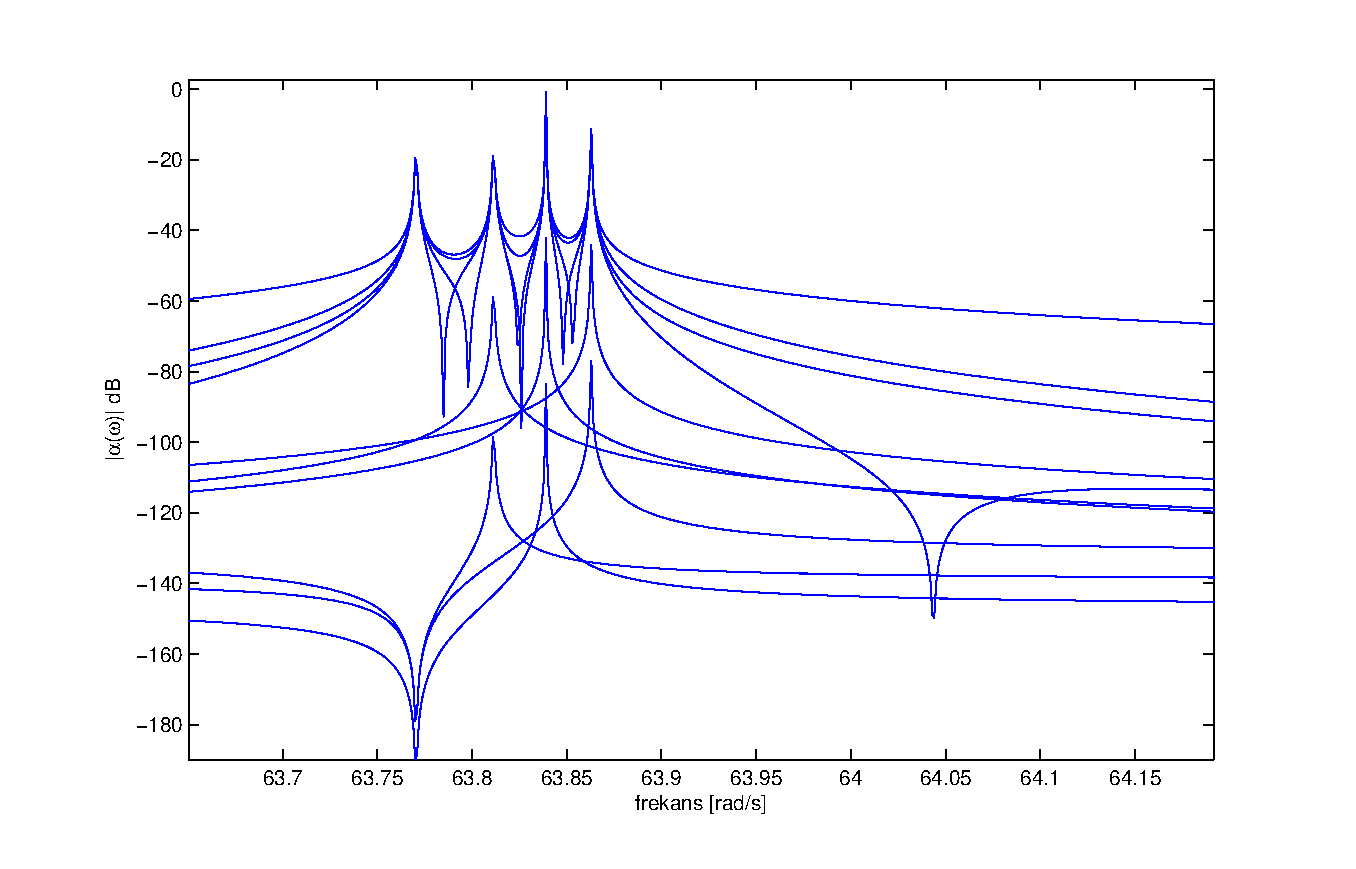
\includegraphics[width=1.3\textwidth]{./reseptanssdBz.eps}}}
\caption[Sönümlü hal reseptans matrisi elemanları]{Sönümlü hal reseptans matrisi elemanlarının $\omega\approx62-63 rad/s$ civarındaki çizgileri. }
\label{fig:reseptanssdbz}
\end{figure}
\clearpage
\subsection*{7. Nokta FRF'leri çizdiriniz.Belirgin özelliklerini bu grafikler yardımıyla izah ediniz.}
Nokta FRF'ler reseptans matrisi diagonal elemanlarıdır. Bunların çizdirilmesiyle;\\
~\\
\underline{Sönümsüz Nokta FRF'ler}\\
~\\
\underline{Tüm modlar:}\\
Tüm modların grafiği Şekil \ref{fig:noktaFRF} 'de verilmiştir. Şekilden görüldüğü üzere modlar iki ayrı grup olmak üzere düşük frekans ve yüksek frekansta yoğunlaşmışlardır. Ayrıca $|\alpha(\omega)_{11}|,|\alpha(\omega)_{22}|,|\alpha(\omega)_{33}|$ lerin düşük frekanslarda tek bir doğal frekansları yakalanmıştır. Bu düşük frekanslarda ilgili serbestlikleri rezonansa sokmanın diğer ilgili serbestlikleri etkilemeyeceğini göstermektedir.
\begin{figure}[H]
\shorthandoff{=}
\centerline{
{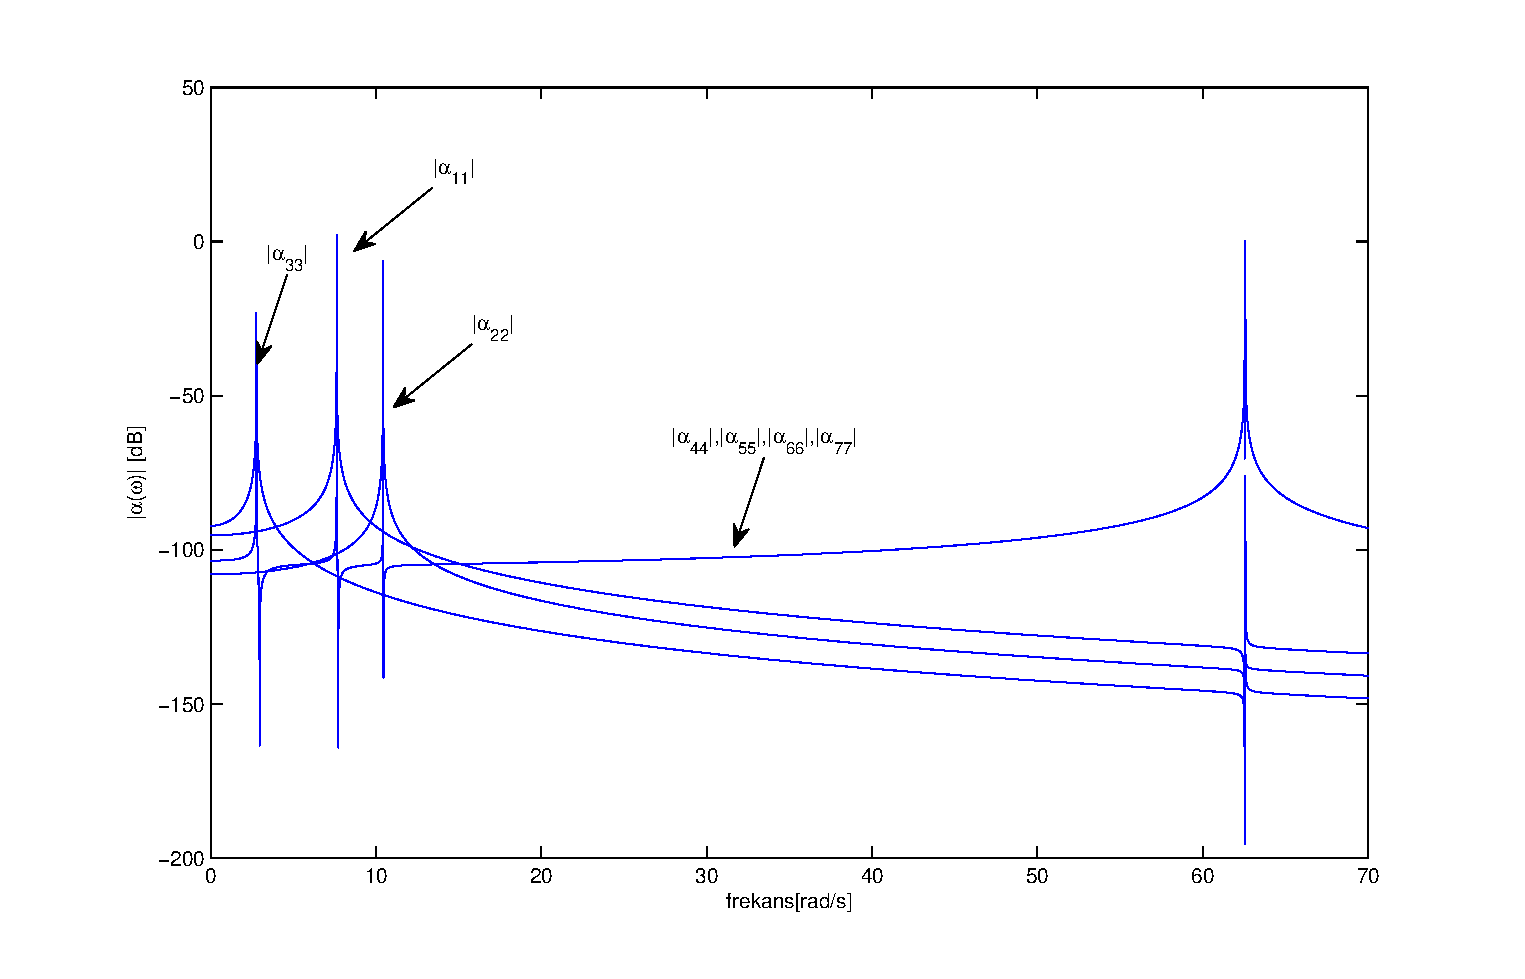
\includegraphics[width=1.3\textwidth]{./noktaFRF.eps}}}
\caption[Sönümsüz hal nokta FRF'ler]{Sönümsüz hal nokta FRF'ler, tüm modlar; yatay eksen ${rad}/{s}$ ve dikey eksen $dB$ }
\label{fig:noktaFRF}
\end{figure}
~\\
\clearpage~\\
\underline{İlk üç mod:}\\
Bu grafikten görülmektedir ki her iki rezonans noktası arasında bir antirezonans bulunmaktadır.
\begin{figure}[H]
\shorthandoff{=}
\centerline{
{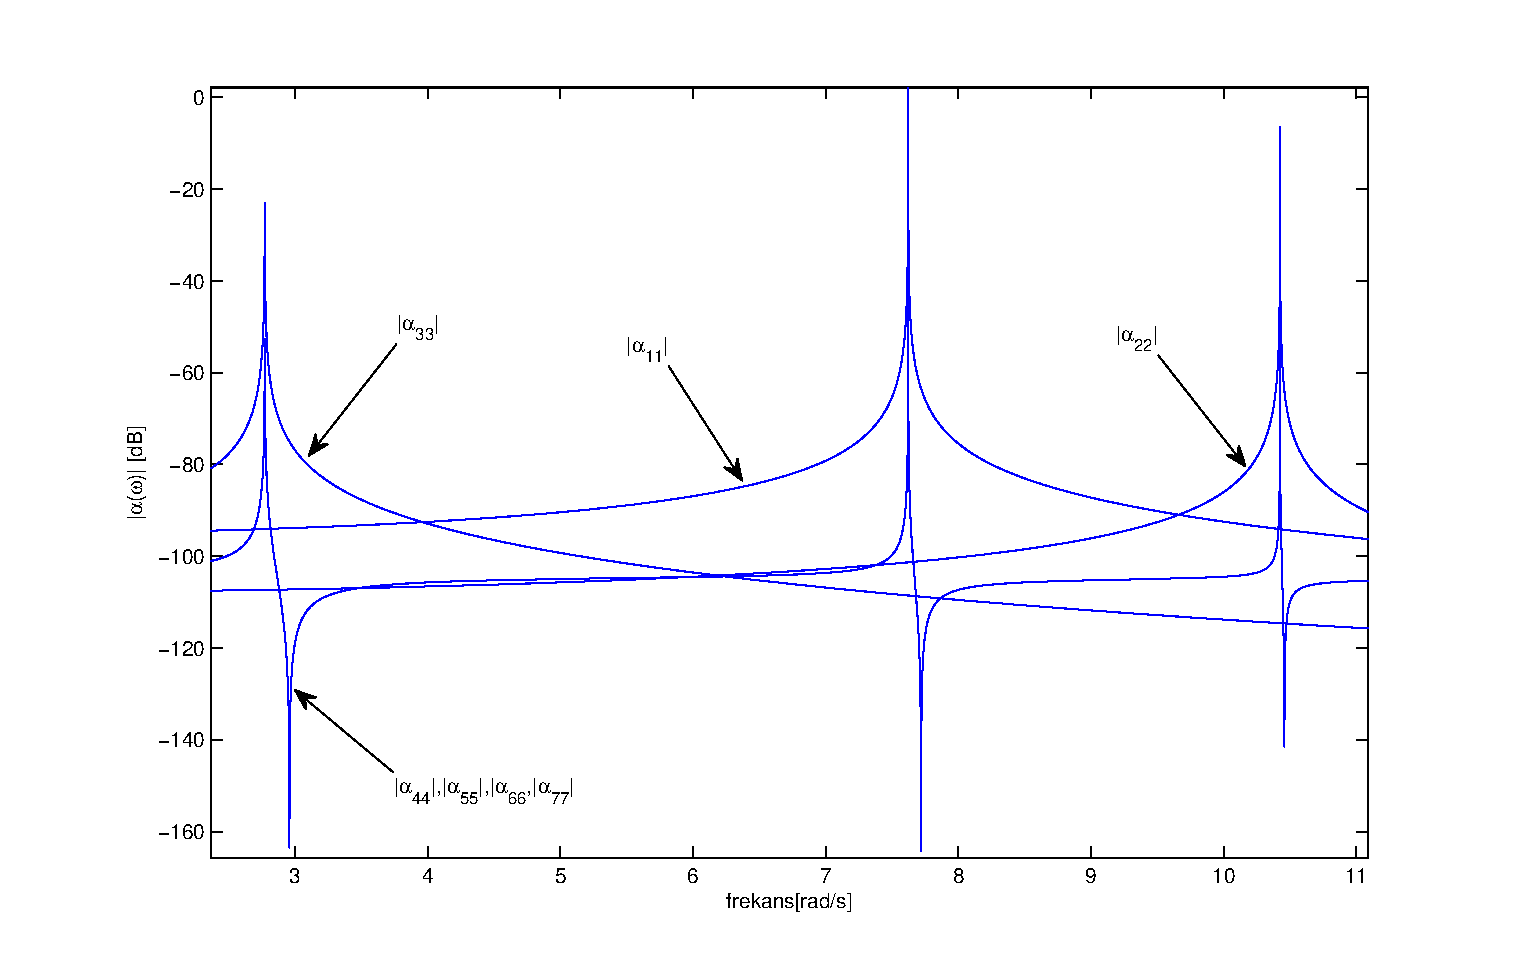
\includegraphics[width=1.3\textwidth]{./noktaFRFmod1-3.eps}}}
~\\

\caption[Sönümsüz hal nokta FRF'ler]{Sönümsüz hal nokta FRF'ler ilk 3 mod; yatay eksen ${rad}/{s}$ ve dikey eksen $dB$ }
\label{fig:noktaFRF1-3}
\end{figure}
~\\
\clearpage~\\
\underline{4-7. modlar:}\\
Grafikten görülmektedir 4.,5.,6.,7. serbestliklere uygulanacak rezonans tahrikleri bir frekans hariç 1.,2.,3. nolu serbestlikleri de rezonansa sokacaktır. O bir adet frekansta da 1.,2.,3. nolu serbestlikler anti rezonans özelliği göstermektedir.
\begin{figure}[H]
\shorthandoff{=}
\centerline{
{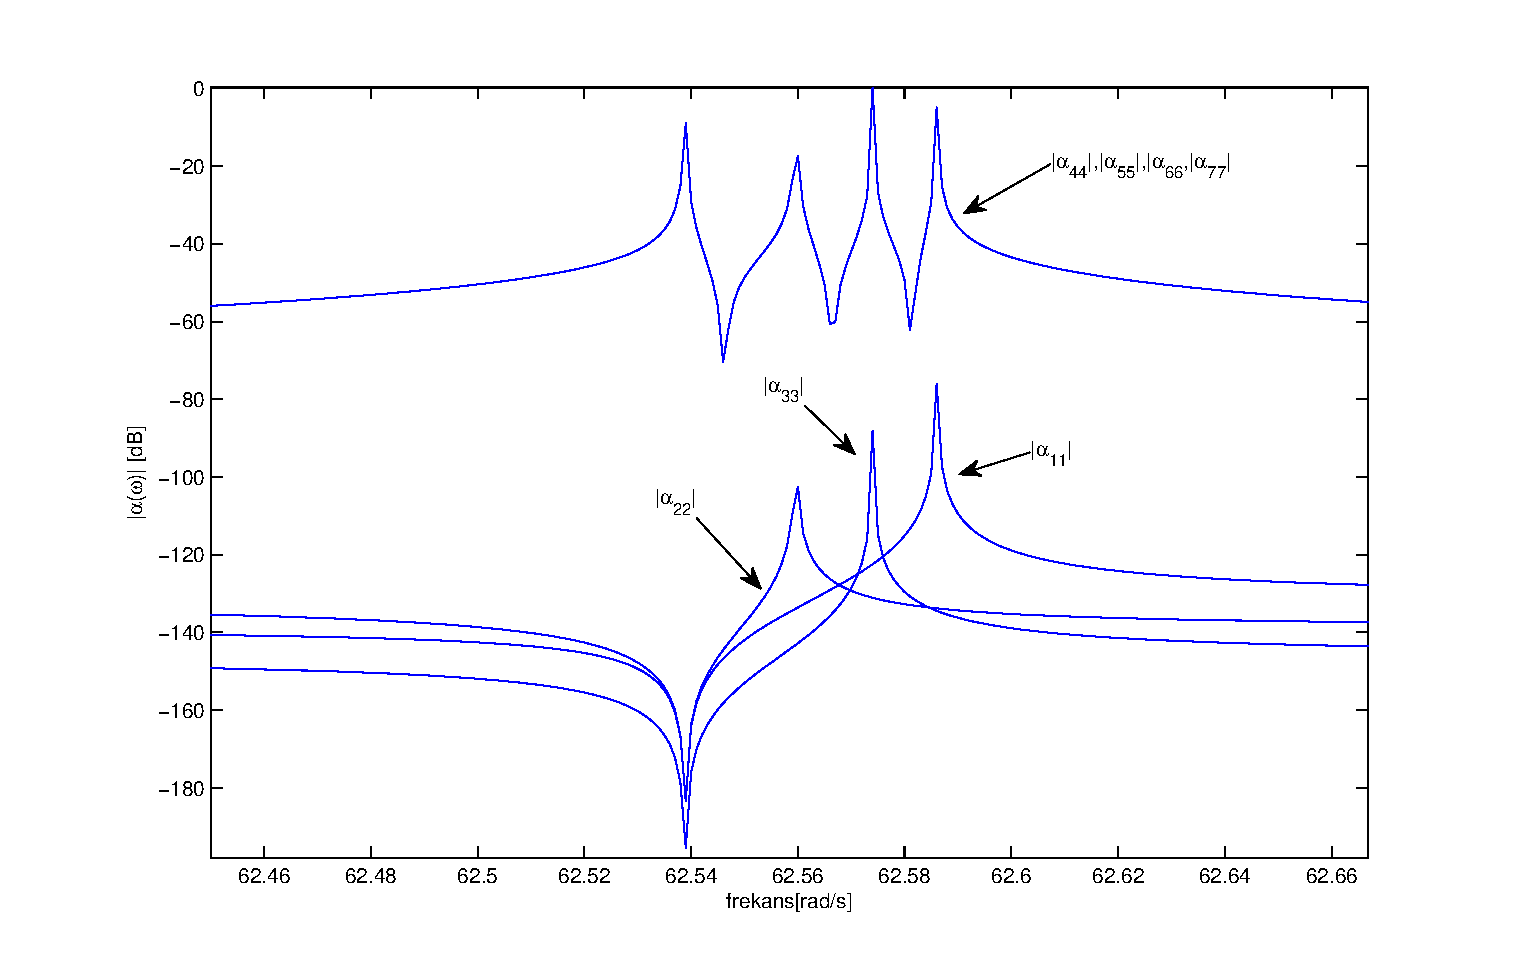
\includegraphics[width=1.3\textwidth]{./noktaFRFmod3-7.eps}}}
\caption[Sönümsüz hal nokta FRF'ler]{Sönümsüz hal nokta FRF'ler  4-7. modlar; yatay eksen ${rad}/{s}$ ve dikey eksen $dB$ }
\label{fig:noktaFRF4-7}
\end{figure}
~\\
~\\\clearpage
~\\
\underline{Sönümlü Nokta FRF'ler:}\\
~\\
Sönümlü halde görüldüğü üzere doğal frekanslar x ekseninde ötelenmiştir. Onun haricinde doğal frekanslar daha yumuşak bir şekilde pik yapmaktadır. \\~\\
\underline{Tüm modlar:}\\
\begin{figure}[H]\shorthandoff{=}
\centerline{
{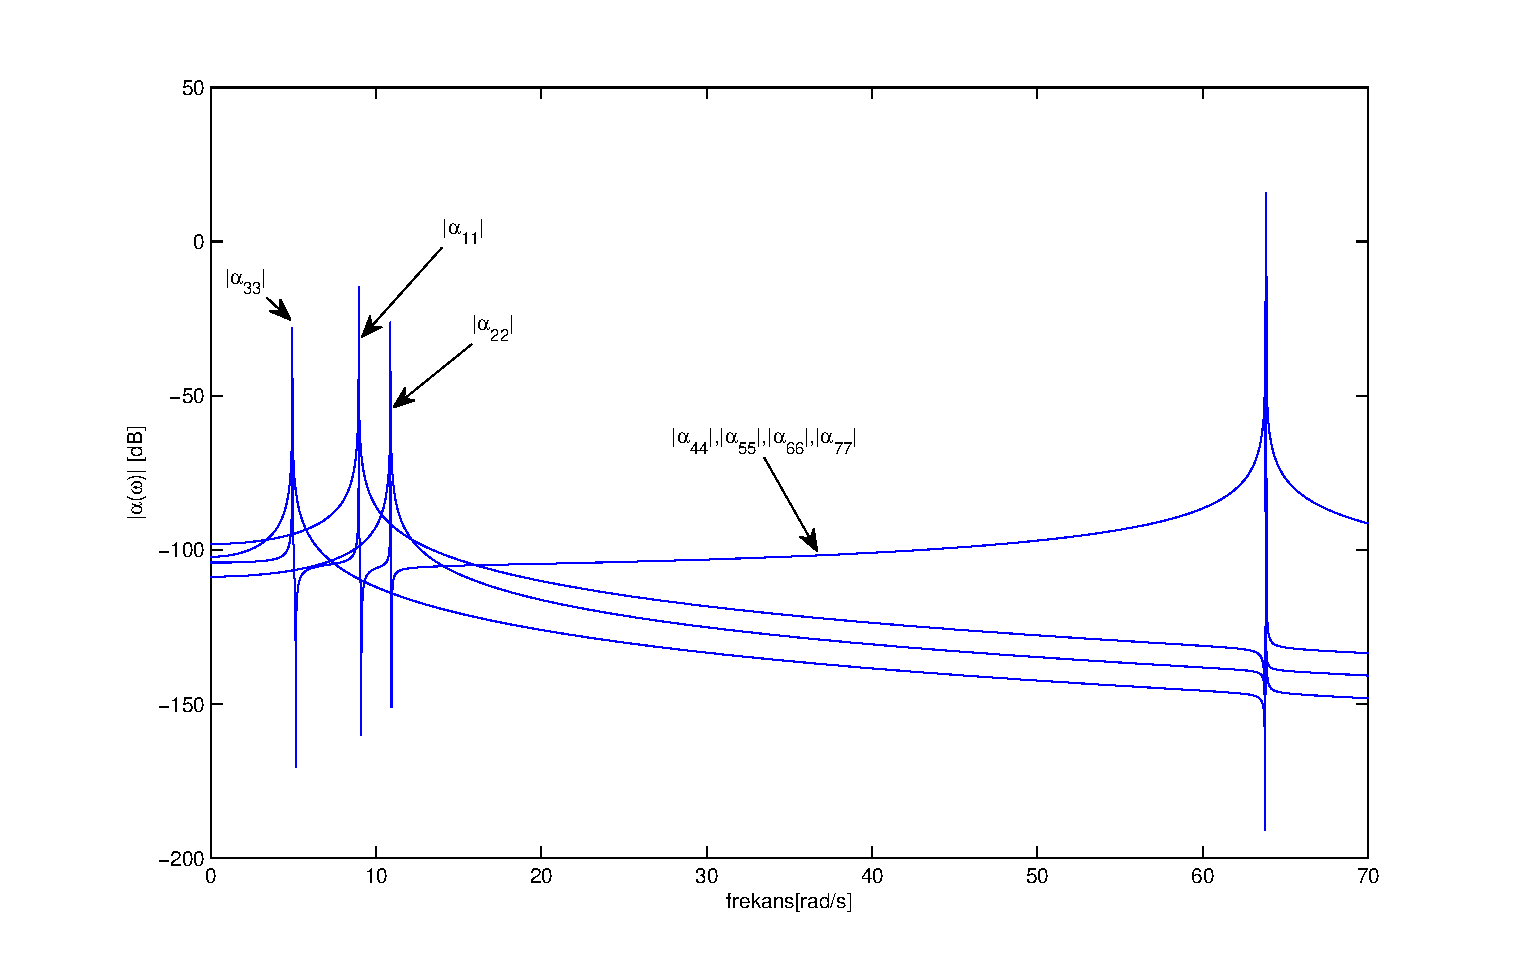
\includegraphics[width=1.3\textwidth]{./noktaFRFs.eps}}}
\caption[Sönümsüz hal nokta FRF'ler]{Sönümlü hal nokta FRF'ler, tüm modlar; yatay eksen ${rad}/{s}$ ve dikey eksen $dB$ }
\label{fig:noktaFRFs}
\end{figure}\clearpage~\\
\underline{İlk üç mod:}\\
\begin{figure}[H]
\shorthandoff{=}
\centerline{
{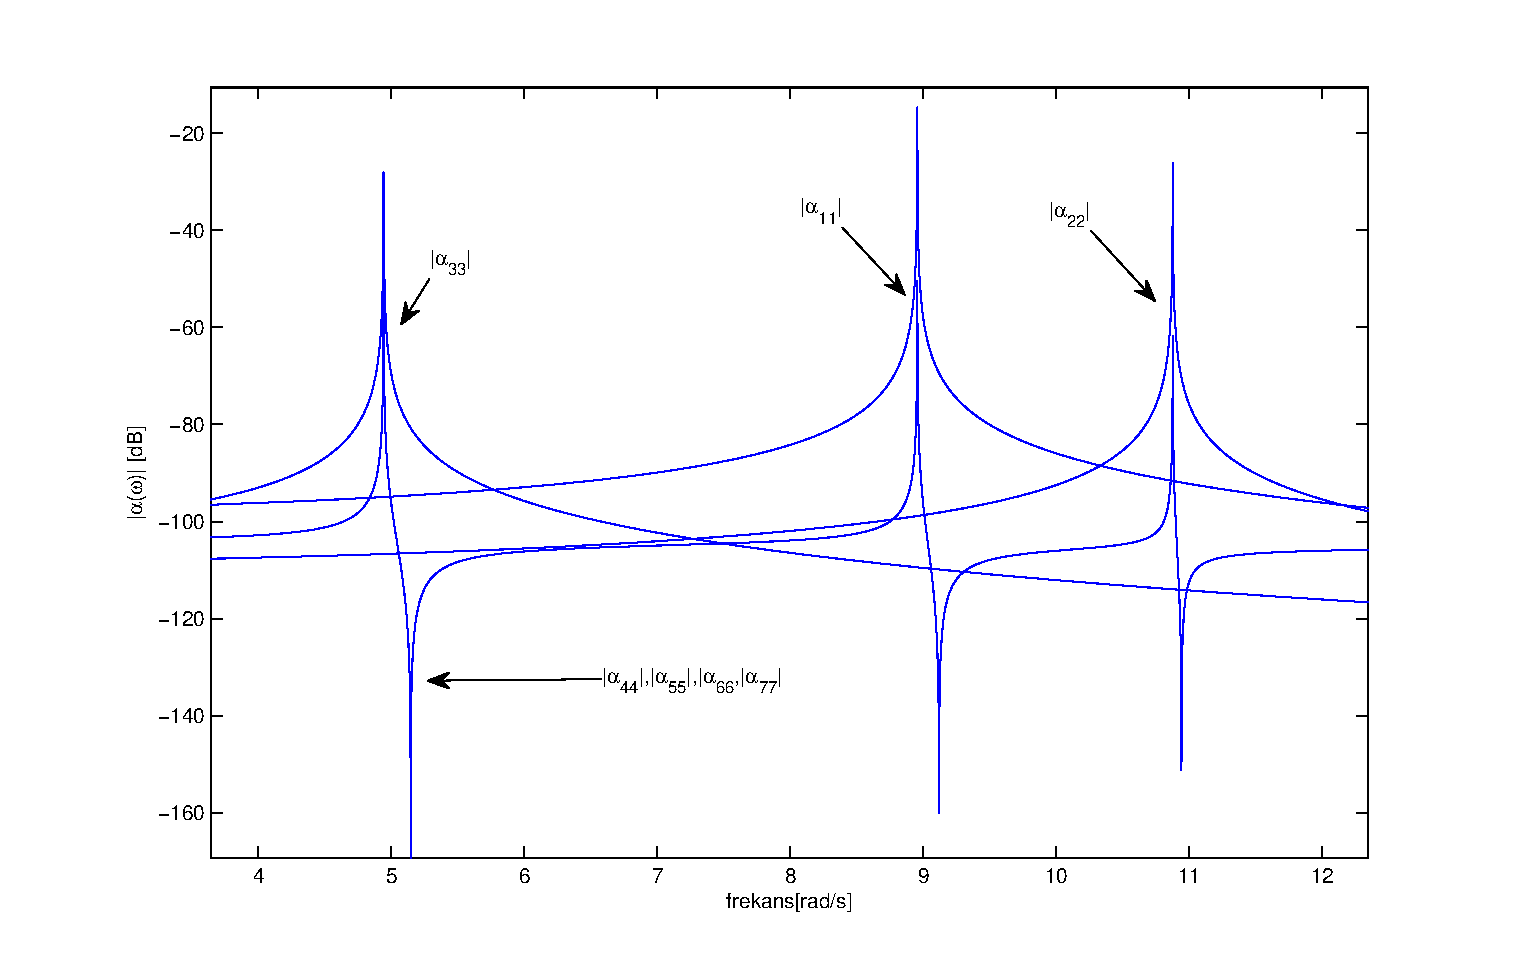
\includegraphics[width=1.3\textwidth]{./noktaFRFsmod1-3.eps}}}
\caption[Sönümsüz hal nokta FRF'ler]{Sönümlü hal nokta FRF'ler ilk 3 mod; yatay eksen ${rad}/{s}$ ve dikey eksen $dB$ }
\label{fig:noktaFRFs1-3}
\end{figure}
\clearpage~\\
\underline{4-7. modlar:}\\
\begin{figure}[H]\shorthandoff{=}
\centerline{
{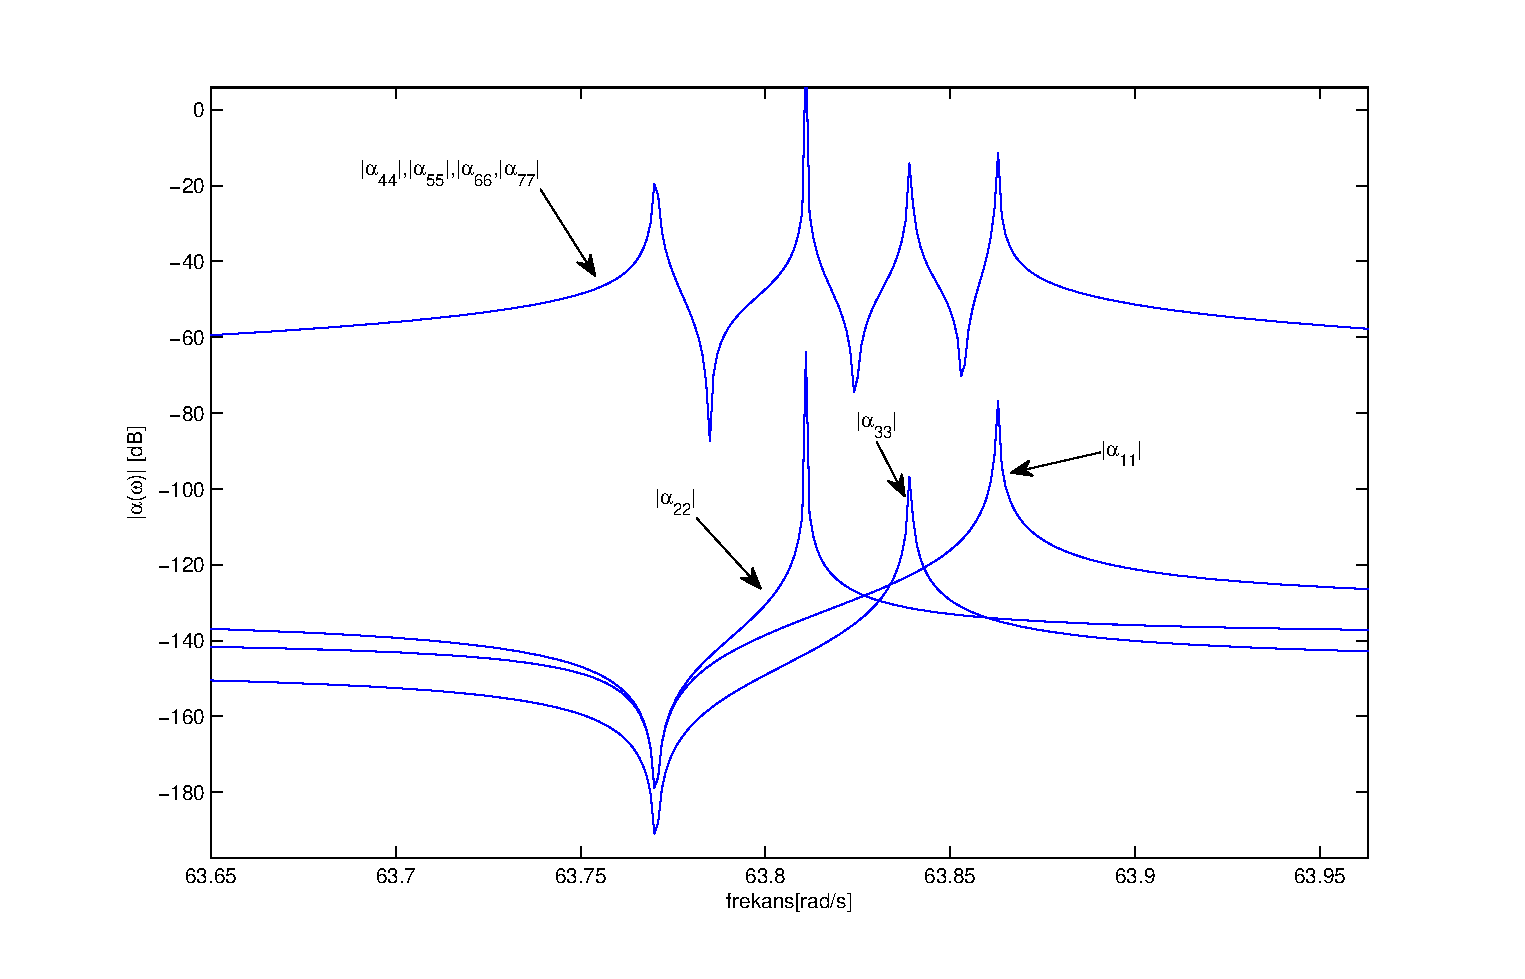
\includegraphics[width=1.3\textwidth]{./noktaFRFsmod3-7.eps}}}
\caption[Sönümsüz hal nokta FRF'ler]{Sönümlü hal nokta FRF'ler  4-7. modlar; yatay eksen ${rad}/{s}$ ve dikey eksen $dB$ }
\label{fig:noktaFRFs4-7}
\end{figure}
\clearpage
\subsection*{8. Transfer FRF'leri çizdiriniz. Belirgin özelliklerini bu grafikler yardımıyla izah ediniz.}
Transfer FRF'ler reseptans matrisinin diagonal olmayan elemanlarıdır. Bunların grafikleri Nokta FRF'ler ile benzer olacaktır. Ancak transfer FRF'ler $\i.$ serbestliğe uygulanan kuvvetin $j.$ serbestlik üzerindeki etkisini göstermektedir. Transfer FRF'lerin çizdirilirse;\\
~\\
\underline{Sönümsüz Transfer FRF'ler}\\
~\\
\underline{Tüm modlar:}\\
\begin{figure}[H]
\shorthandoff{=}
\centerline{
{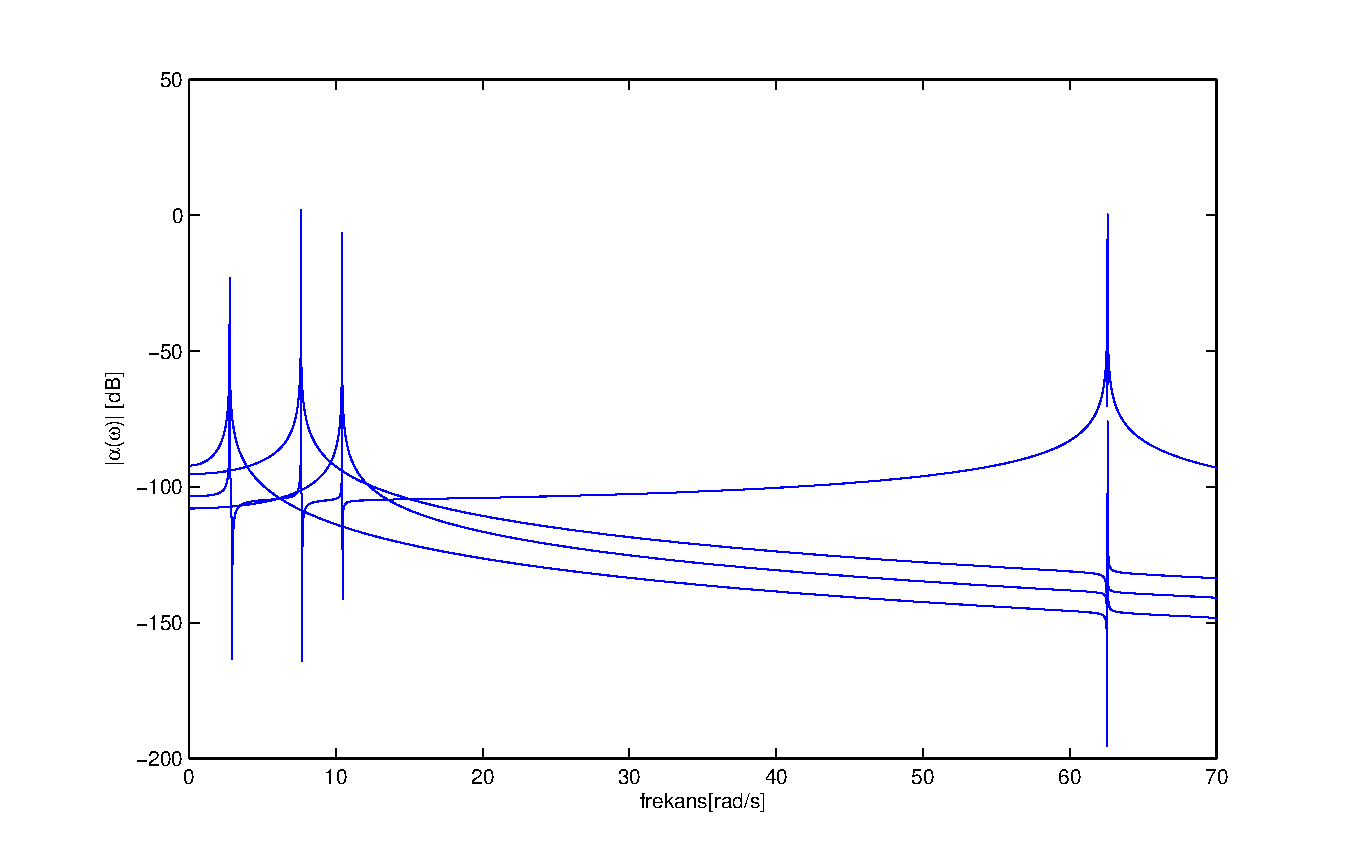
\includegraphics[width=1.3\textwidth]{./transferFRF.eps}}}
\caption[Sönümsüz hal nokta FRF'ler]{Sönümsüz hal nokta FRF'ler, tüm modlar; yatay eksen ${rad}/{s}$ ve dikey eksen $dB$ }
\label{fig:noktaFRF}
\end{figure}
~\\
\clearpage~\\
\underline{İlk üç mod:}\\
\begin{figure}[H]
\shorthandoff{=}
\centerline{
{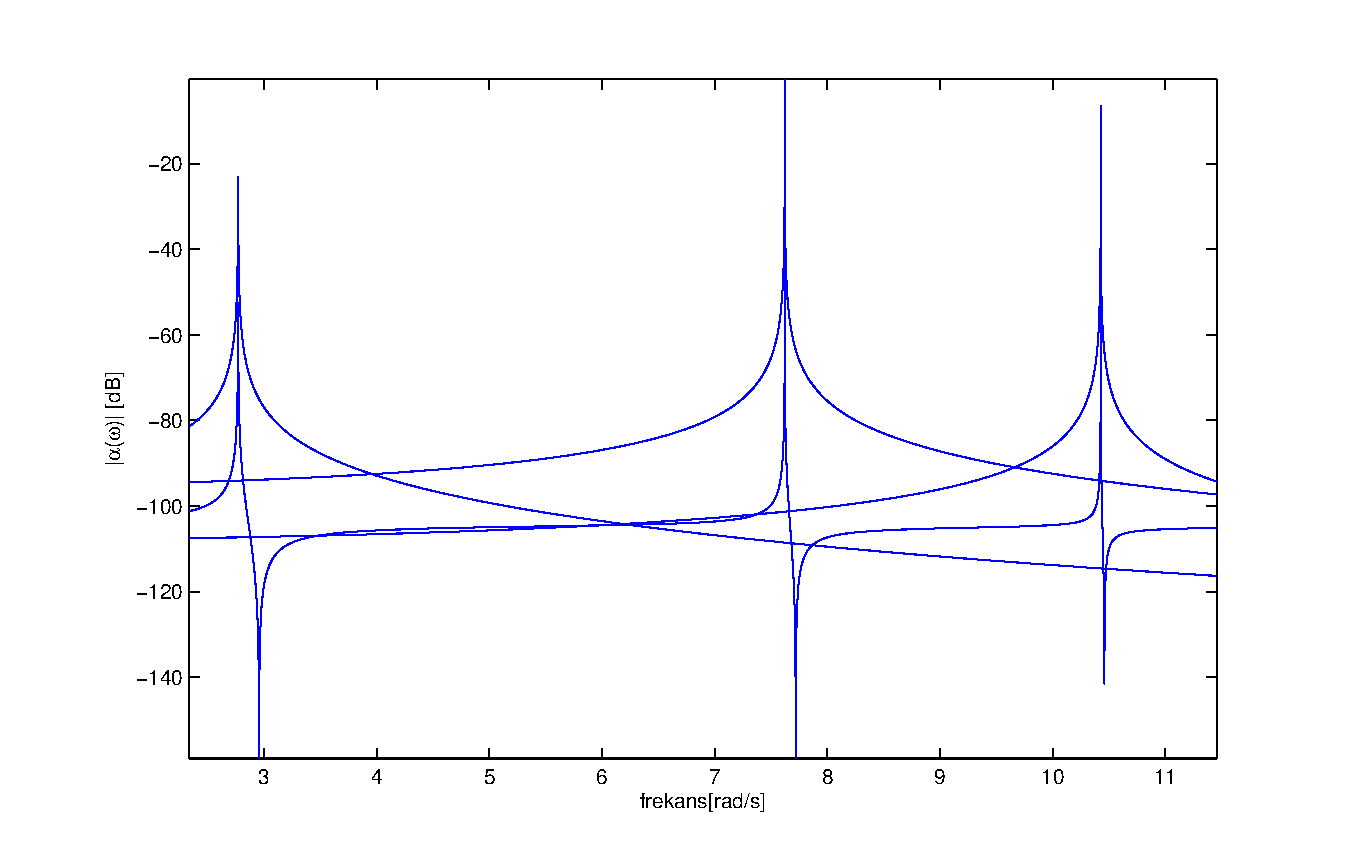
\includegraphics[width=1.3\textwidth]{./transferFRF1-3.eps}}}
~\\

\caption[Sönümsüz hal nokta FRF'ler]{Sönümsüz hal nokta FRF'ler ilk 3 mod; yatay eksen ${rad}/{s}$ ve dikey eksen $dB$ }
\label{fig:noktaFRF1-3}
\end{figure}
~\\
\clearpage~\\
\underline{4-7. modlar:}\\
\begin{figure}[H]
\shorthandoff{=}
\centerline{
{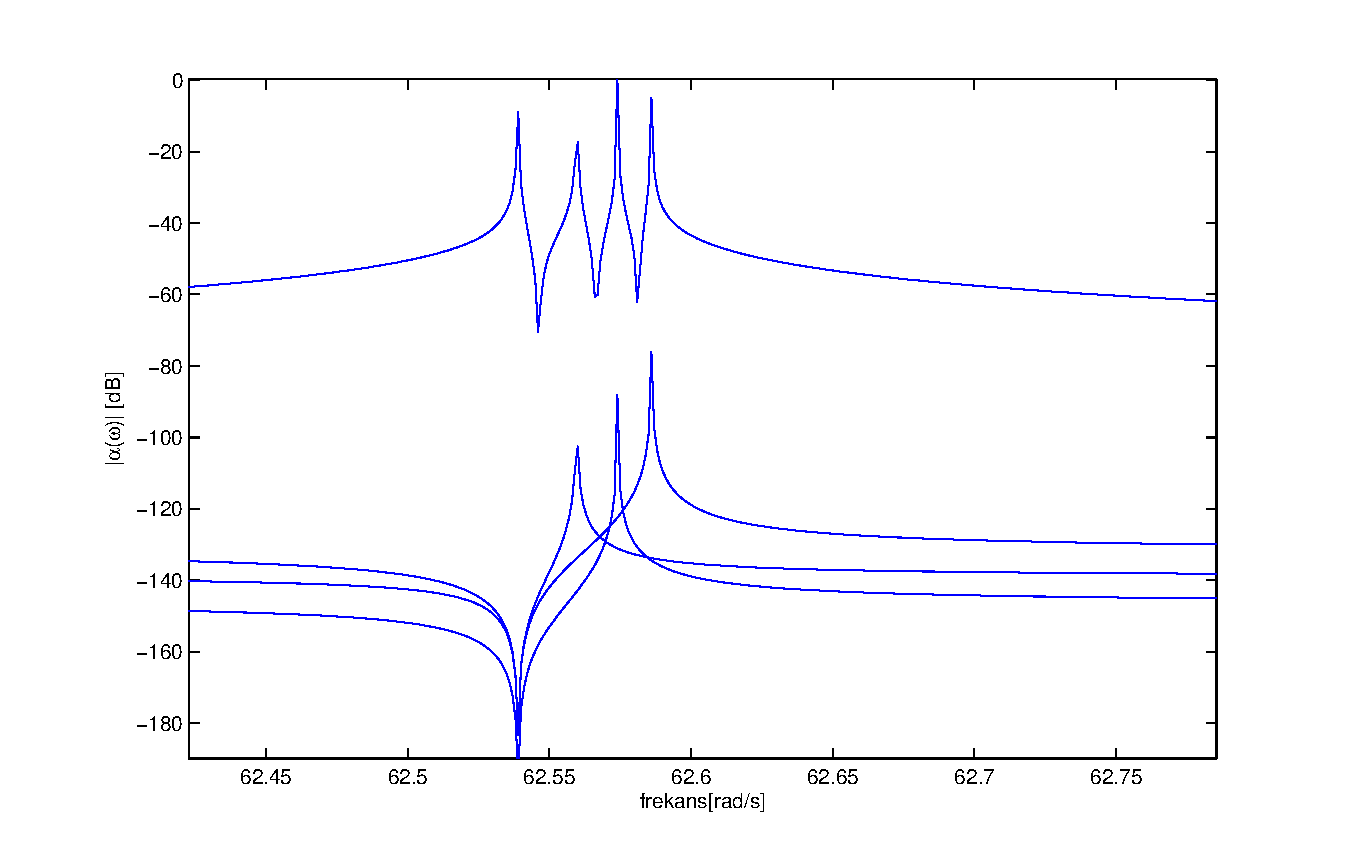
\includegraphics[width=1.3\textwidth]{./transferFRF3-6.eps}}}
\caption[Sönümsüz hal nokta FRF'ler]{Sönümsüz hal nokta FRF'ler  4-7. modlar; yatay eksen ${rad}/{s}$ ve dikey eksen $dB$ }
\label{fig:noktaFRF4-7}
\end{figure}
~\\
~\\\clearpage
~\\
\underline{Sönümlü Nokta FRF'ler:}\\
~\\
\\~\\
\underline{Tüm modlar:}\\
\begin{figure}[H]\shorthandoff{=}
\centerline{
{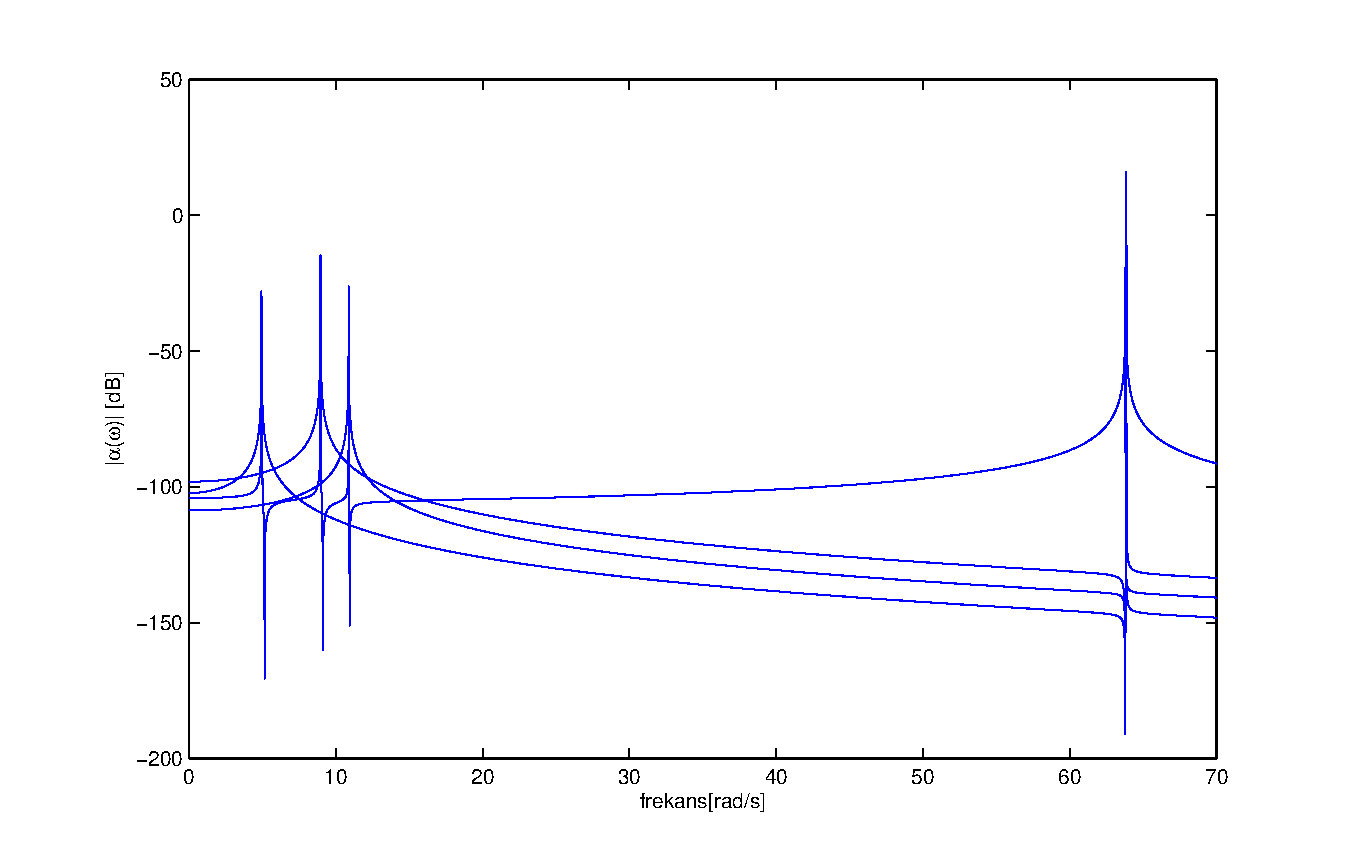
\includegraphics[width=1.3\textwidth]{./transferFRFs.eps}}}
\caption[Sönümsüz hal nokta FRF'ler]{Sönümlü hal nokta FRF'ler, tüm modlar; yatay eksen ${rad}/{s}$ ve dikey eksen $dB$ }
\label{fig:noktaFRFs}
\end{figure}\clearpage~\\
\underline{İlk üç mod:}\\
\begin{figure}[H]
\shorthandoff{=}
\centerline{
{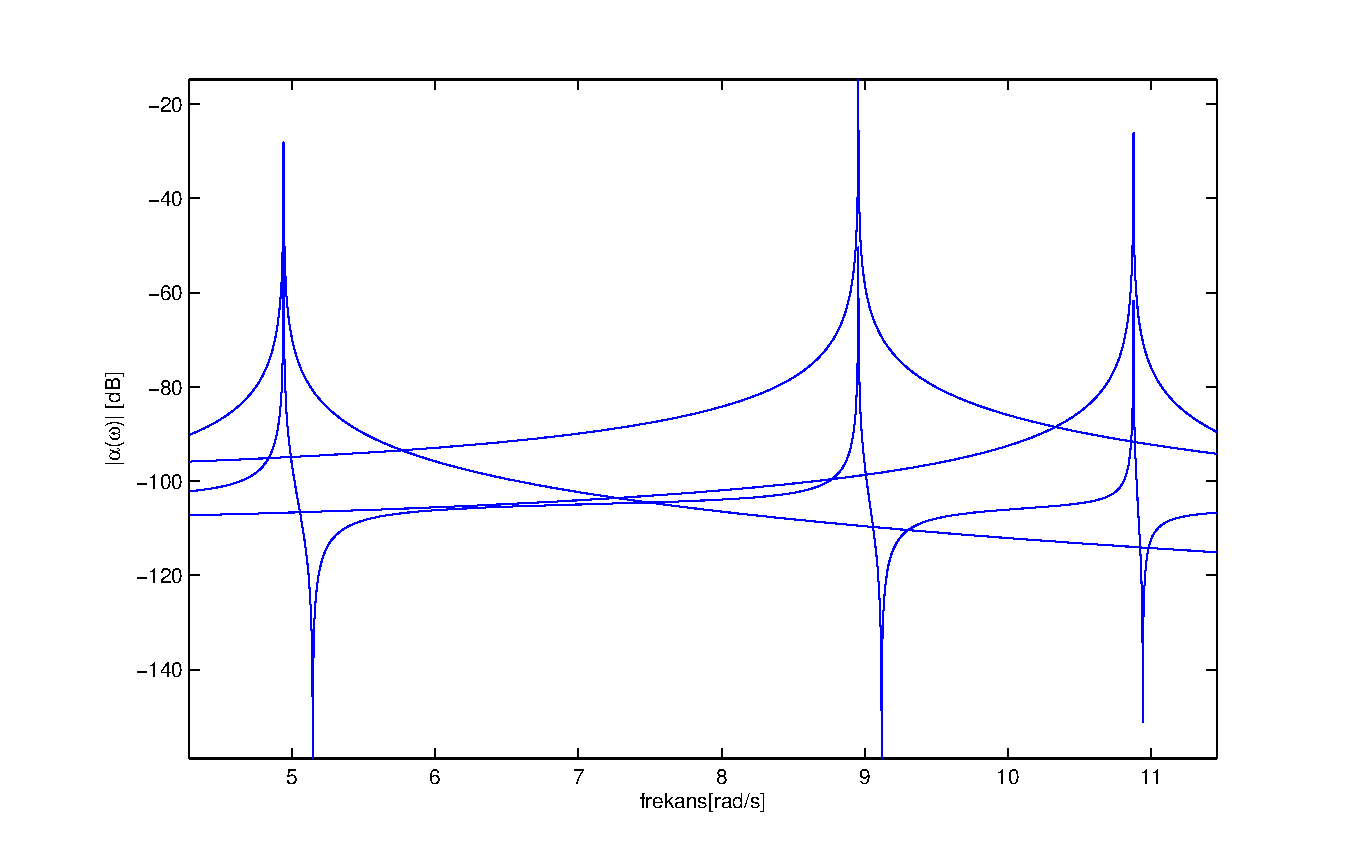
\includegraphics[width=1.3\textwidth]{./transferFRFs1-3.eps}}}
\caption[Sönümsüz hal nokta FRF'ler]{Sönümlü hal nokta FRF'ler ilk 3 mod; yatay eksen ${rad}/{s}$ ve dikey eksen $dB$ }
\label{fig:noktaFRFs1-3}
\end{figure}
\clearpage~\\
\underline{4-7. modlar:}\\
\begin{figure}[H]\shorthandoff{=}
\centerline{
{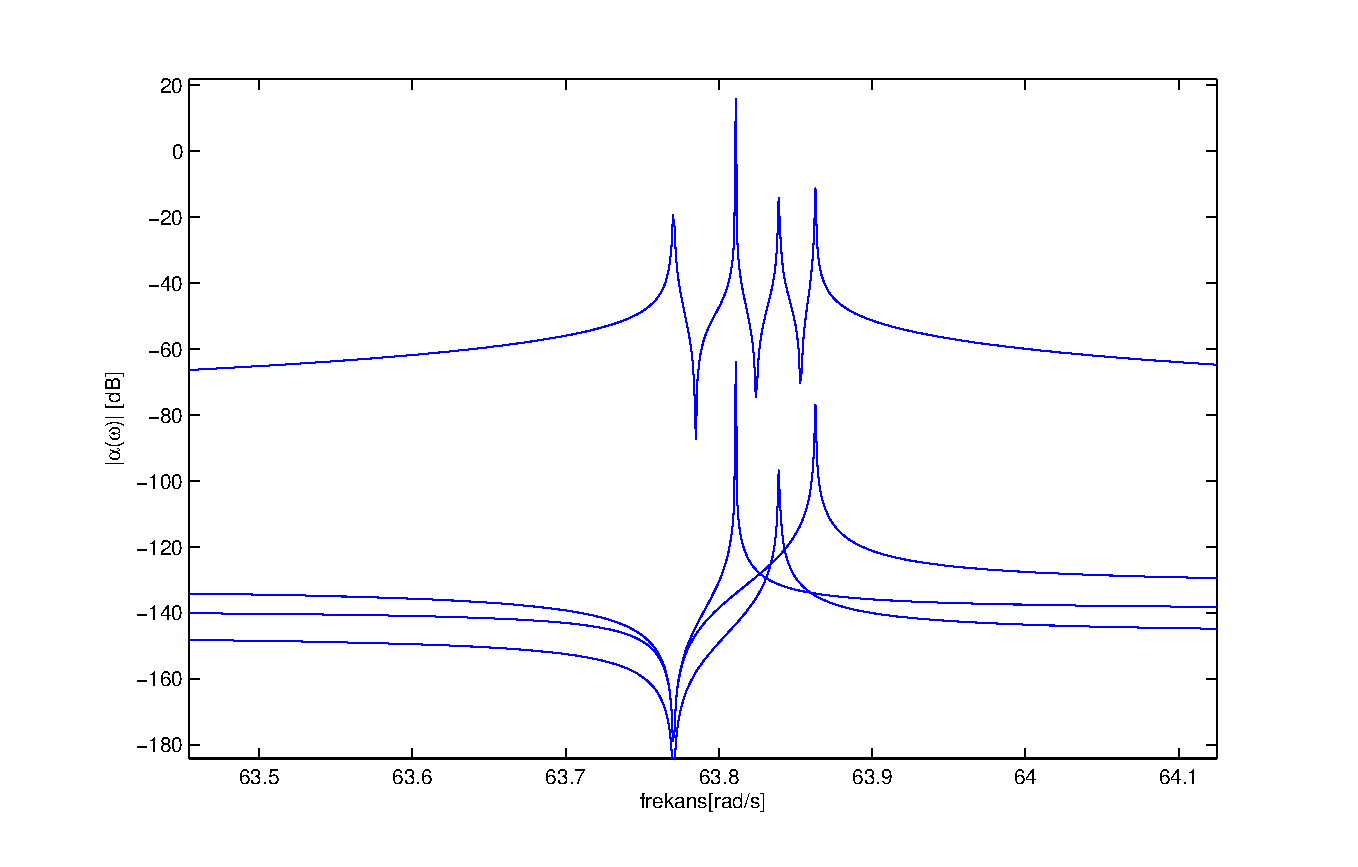
\includegraphics[width=1.3\textwidth]{./transferFRFs3-6.eps}}}
\caption[Sönümsüz hal nokta FRF'ler]{Sönümlü hal transfer FRF'ler  4-7. modlar; yatay eksen ${rad}/{s}$ ve dikey eksen $dB$ }
\label{fig:noktaFRFs4-7}
\end{figure}

\clearpage
\subsection*{9. Tüm mobilite eğrilerini tek bir grafikte topluca çizdiriniz.}
~\\
\underline{Sönümsüz hal mobilite eğrileri:}\\
~\\
\begin{figure}[H]\shorthandoff{=}
\centerline{
{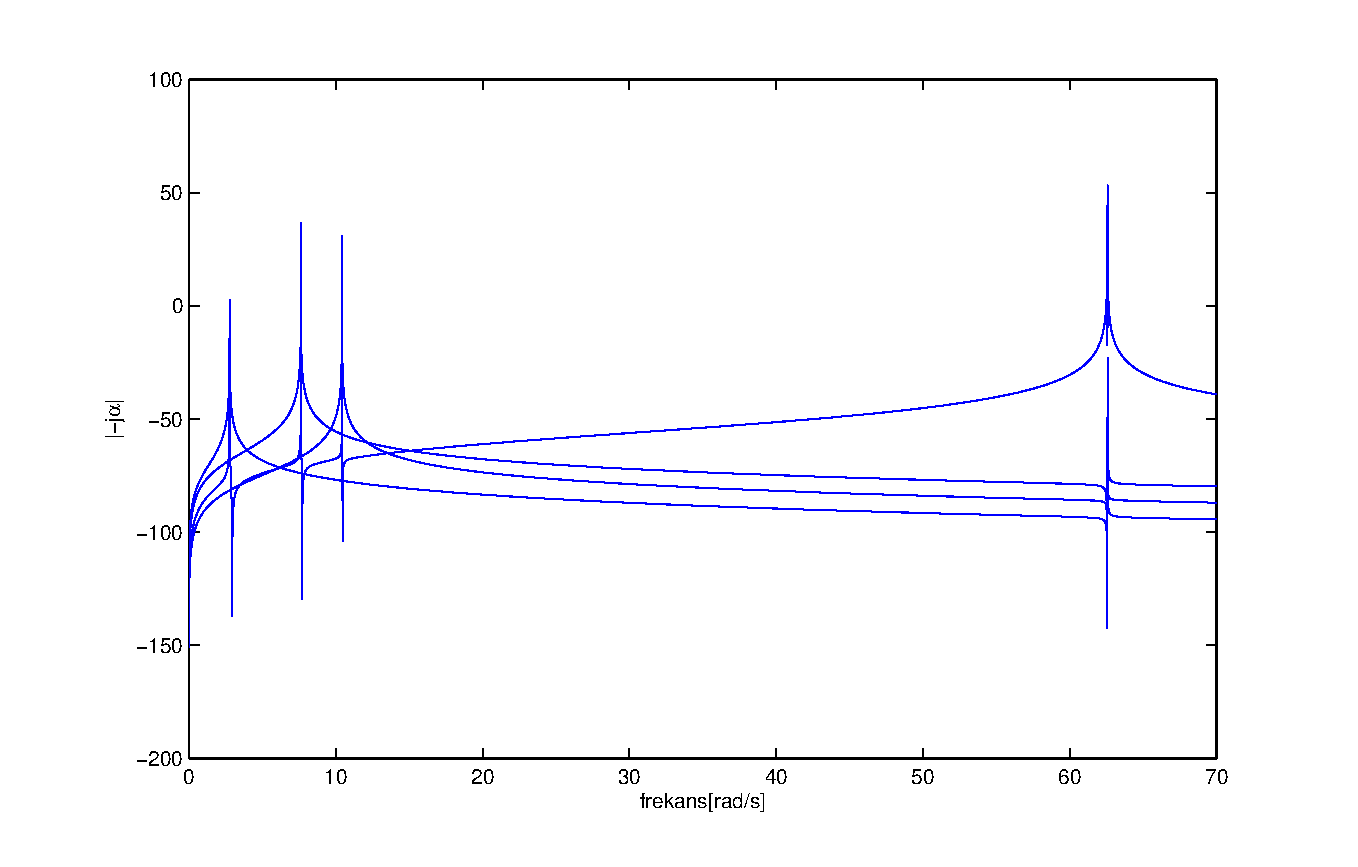
\includegraphics[width=1.3\textwidth]{./mobilite.eps}}}
\caption[Sönümsüz hal nokta FRF'ler]{Sönümsüz hal tüm mobilite eğrileri; yatay eksen ${rad}/{s}$ ve dikey eksen $dB$ }
\label{fig:noktaFRFs4-7}
\end{figure}
~\\\clearpage~\\
\underline{Sönümlü hal mobilite eğrileri:}\\
~\\
\begin{figure}[H]\shorthandoff{=}
\centerline{
{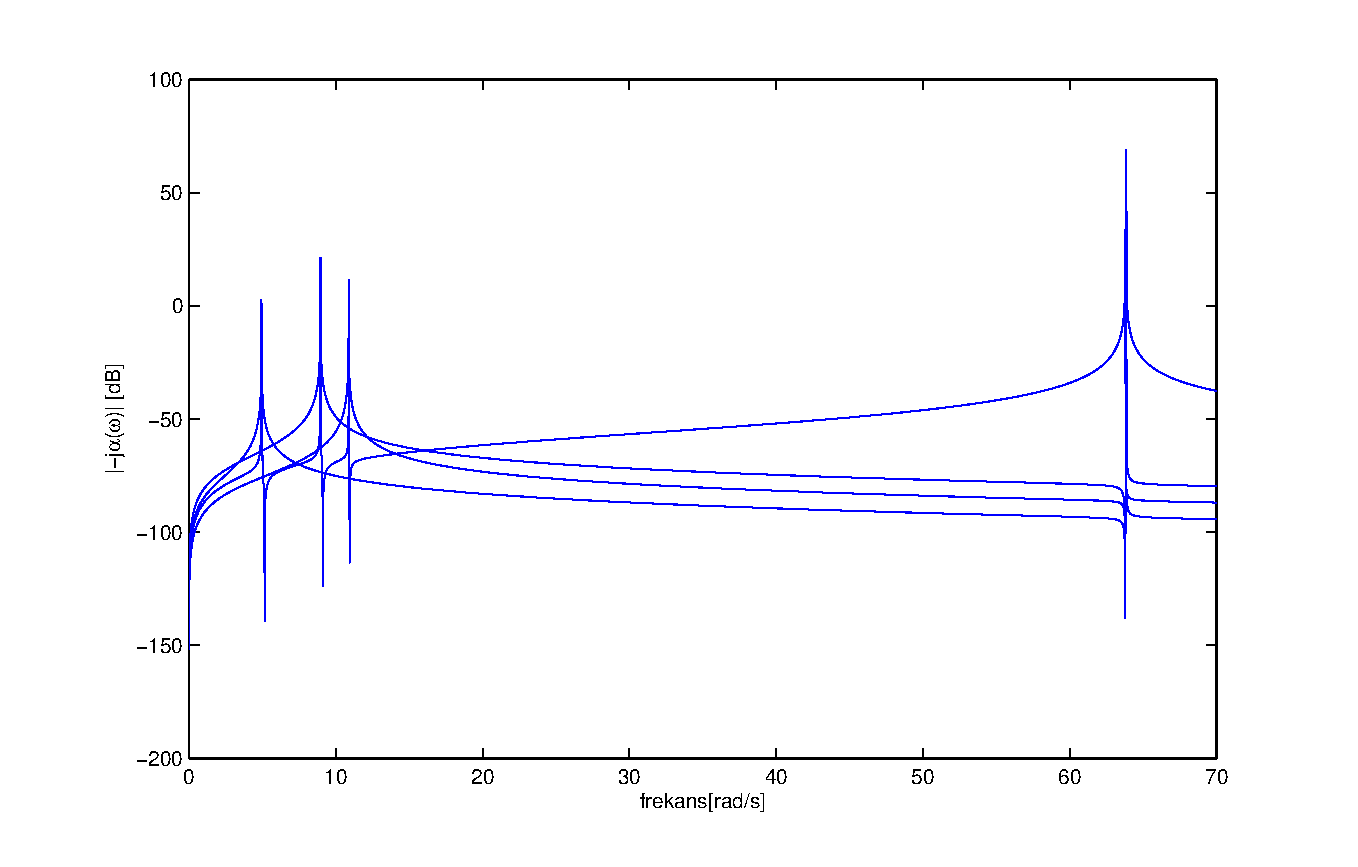
\includegraphics[width=1.3\textwidth]{./mobilites.eps}}}
\caption[Sönümsüz hal nokta FRF'ler]{Sönümlü hal tüm mobilirte eğrileri; yatay eksen ${rad}/{s}$ ve dikey eksen $dB$ }
\label{fig:noktaFRFs4-7}
\end{figure}
~\\\clearpage~\\
\underline{Sönümsüz hal akselerans eğrileri:}\\
~\\
\begin{figure}[H]\shorthandoff{=}
\centerline{
{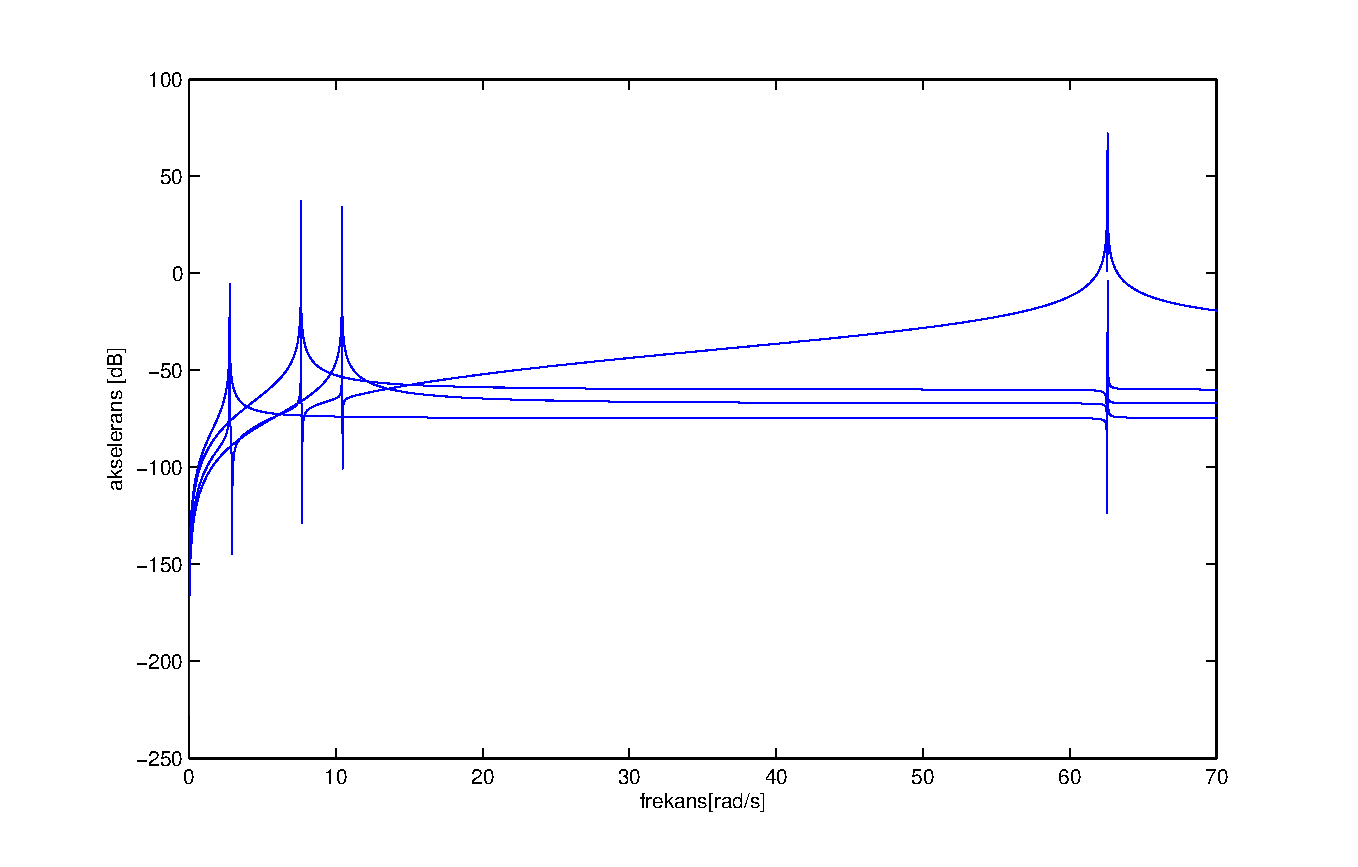
\includegraphics[width=1.3\textwidth]{./akselerans.eps}}}
\caption[Sönümsüz hal nokta FRF'ler]{Sönümsüz hal tüm mobilite eğrileri; yatay eksen ${rad}/{s}$ ve dikey eksen $dB$ }
\label{fig:noktaFRFs4-7}
\end{figure}
~\\\clearpage~\\
\underline{Sönümlü hal akselerans eğrileri:}\\
~\\
\begin{figure}[H]\shorthandoff{=}
\centerline{
{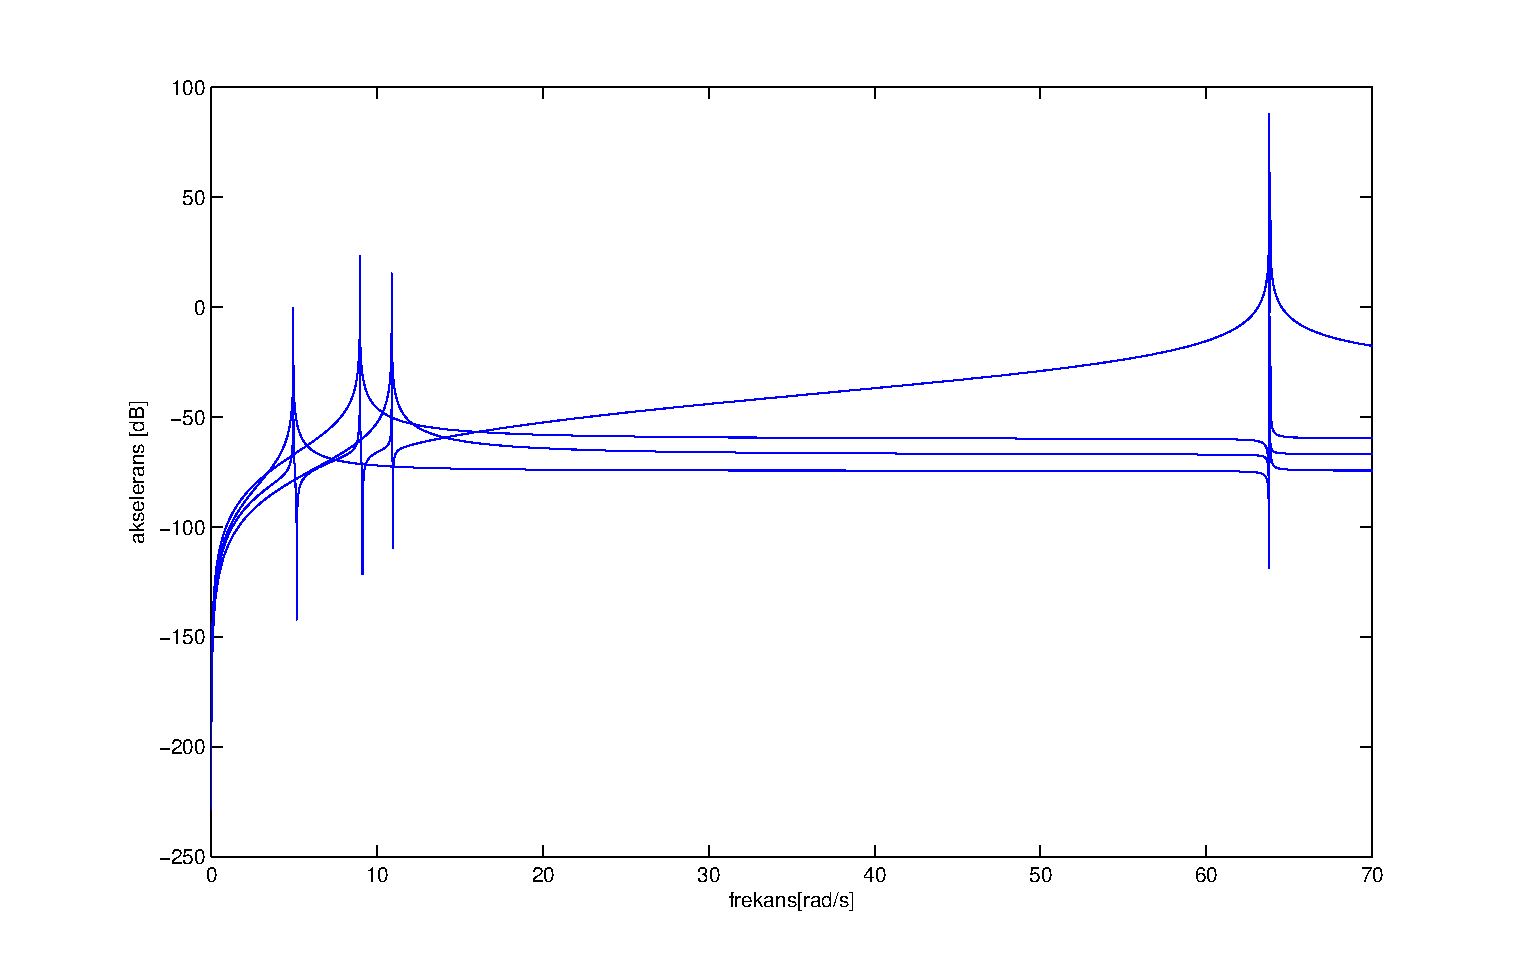
\includegraphics[width=1.3\textwidth]{./akseleranss.eps}}}
\caption[Sönümsüz hal nokta FRF'ler]{Sönümlü hal tüm mobilirte eğrileri; yatay eksen ${rad}/{s}$ ve dikey eksen $dB$ }
\label{fig:noktaFRFs4-7}
\end{figure}

\end{document}          
